% ****** Start of file apssamp.tex ******
%
%   This file is part of the APS files in the REVTeX 4.2 distribution.
%   Version 4.2a of REVTeX, December 2014
%
%   Copyright (c) 2014 The American Physical Society.
%
%   See the REVTeX 4 README file for restrictions and more information.
%
% TeX'ing this file requires that you have AMS-LaTeX 2.0 installed
% as well as the rest of the prerequisites for REVTeX 4.2
%
% See the REVTeX 4 README file
% It also requires running BibTeX. The commands are as follows:
%
%  1)  latex apssamp.tex
%  2)  bibtex apssamp
%  3)  latex apssamp.tex
%  4)  latex apssamp.tex
%
\documentclass[%
 reprint,
%superscriptaddress,
%groupedaddress,
%unsortedaddress,
%runinaddress,
%frontmatterverbose, 
%preprint,
%preprintnumbers,
%nofootinbib,
%nobibnotes,
%bibnotes,
 amsmath,amssymb,
 aps,
%pra,
prb,
%rmp,
%prstab,
%prstper,
floatfix,
]{revtex4-2}

%\newcommand*{\INTERNAL}{}

\usepackage{graphicx}% Include figure files
\usepackage{dcolumn}% Align table columns on decimal point
\usepackage{bm}% bold math
\usepackage{hyperref}% add hypertext capabilities
\hypersetup{colorlinks=true,urlcolor={blue},citecolor={blue}, linkcolor={blue}}
\usepackage{amsmath} % or simply amstext
%\newcommand{\angstrom}{\textup{\angstrom}}
\usepackage{siunitx}
\usepackage{color}
\usepackage[normalem]{ulem}
\usepackage{diagbox}
\usepackage{import}
\usepackage{multirow}
\usepackage{xr} % referencing across multiple files
\usepackage{cleveref} % cite figures in SI
\usepackage[dvipsnames]{xcolor}

%\usepackage{url}            % simple URL typesetting
%\usepackage[mathlines]{lineno}% Enable numbering of text and display math
%\linenumbers\relax % Commence numbering lines
%\usepackage{nameref}

%\usepackage[showframe,%Uncomment any one of the following lines to test 
%%scale=0.7, marginratio={1:1, 2:3}, ignoreall,% default settings
%%text={7in,10in},centering,
%%margin=1.5in,
%%total={6.5in,8.75in}, top=1.2in, left=0.9in, includefoot,
%%height=10in,a5paper,hmargin={3cm,0.8in},
%]{geometry}

\ifdefined\INTERNAL

\newcommand{\lock}{\color{red}}
\newcommand{\zhzh}{\color{blue}}

\else

\newcommand{\lock}{\color{black}}
\newcommand{\zhzh}{\color{blue}}

\fi
%\newcommand{\comm}{\color{Purple}} %comment
\newcommand{\comm}{\color{ForestGreen}} %comment

\newcommand{\sinfo}{Supplementary Information}
% Use Supp Info labels with SI- prefix
\externaldocument[SI-]{SI}

\begin{document}

\title{Role of adatoms in the coupling of phenyl groups on Cu(111) surface}

\author{Zhenzhe Zhang}
\author{Dmitrii F. Perepichka}%
\email{dmitrii.perepichka@mcgill.ca}
\author{Rustam Z. Khaliullin}
\email{rustam.khaliullin@mcgill.ca}
\affiliation{%
 Department of Chemistry, McGill University, 801 Sherbrooke St West, Montreal, QC H3A 0B8, Canada
}%

%\date{\today}% It is always \today, today,
             %  but any date may be explicitly specified

\begin{abstract}


There is a mounting evidence from experimental and modeling studies that metal atoms can be raised above or completely extracted from a metal surface during the on-surface Ullmann reaction. In this work, the energetics of the adatom creation during the coupling of two phenyl groups on Cu(111) surface is examined for the first time using DFT modeling. More importantly, previously unstudied effects of adatoms, extracted and pre-existing, on the coupling of two phenyl groups are investigated in detail.
%The results indicate that 
%This manuscript reviews the results of experimental and computational studies of the surface Ullmann coupling that shed light on the role of surface adatoms in its mechanism. A particular focus is on the early stages of the polymerization and coupling of two monomers.
\end{abstract}

\maketitle

%\tableofcontents

%RZK. What a variety of labels mean. 
%RYK - to be replaced with the actual value later
%R1111 or RZKmmdd - mm denotes month, dd - denotes day
%RZKX - these are low priority comments, which will be promoted to regular labels later 
%RZZK - ignore! These labels keep track of my own revision process

%%% GENERAL REMARKS %%%

%RZK: Detailed description of the figure. Take a look at the original publication. Reprinted from~\cite{RZK} with permission of American Chemical Society or PUBLISHER. See the LaTeX comment below. If you take a figure from a publication it is very important to cite the work and obtain publisher's permission. We need to make sure that all our borrowed figures satisfy copyright permissions. For example, see: https://www.stm-assoc.org/2016_01_05_Guidelines_for_Quotation_From_Journal_Articles.pdf

\ifdefined\INTERNAL

Color-coding: 

{\lock RZK and ZZ contributed and agree.}

{\comm Some in-line comments by RZK.}

\textcolor{blue}{Written by ZZ, to be reviewed by RZK.}

{Unclassified text.}

Zhenzhe, if you edit the red text, please save the original as a LaTeX comment. I often need to revert your changes and it takes too much time.

\fi

\section{Introduction}

%RZK0423: The detailed review of the classical Ullmann reaction is saved in the branch named Review-Intro. Dima's comments from January 2021 have not been fully incorporated into the saved version.

%RZK0602: All abbreviations (such as DFT, STM, AFM) must be properly introduced.

%\subsection{On-surface Ullmann coupling}

{\lock

%RZZK: Dima's comment: ``Discuss GNRs and 2D polymers, give some key figures - to tell the reader why they should care to read the rest of the paper.'' I think figures will be useful in the thesis but not in the research article.

Unique and tunable properties of $\pi$-conjugated organic polymers such as one-dimensional (1D) graphene nanoribbons~\cite{ullmann_106, ullmann_45, ullmann_107, ullmann_101}
and two-dimensional (2D) covalent organic frameworks 
%{\comm [RZK0506: check whether the references are suitable for 2D $\pi$-conjugated COFs~\cite{ullmann_108, ullmann_109}]} 
make them promising candidates to produce a variety of electronic and optoelectronic devices~\cite{ullmann_113, ullmann_114}.
%
The utilization of these materials in devices requires scalable methods to create extended polymer structures with low defect density.
%
%RZK0506: On-surface polymerization is a rapidly-developing field aimed at achieving the constructions of unprecedented 1D or 2D polymers with novel structures and revolutionary properties\cite{ullmann_105, ullmann_33, ullmann_70}. 
The on-surface Ullmann reaction is currently viewed as a promising bottom-up strategy to assemble, in mild conditions, atomically precise $\pi$-conjugated organic polymers with high degree of control over their electronic properties~\cite{ullmann_33}. 
%
%A recent surge of interest in electronic devices based on low-dimensional organic nanostructures with $\pi$-conjugated backbones has led to a renewed attention to the Ullmann process.
%The recent surge of interest in bottom-up fabrication of functional nanostructures on surfaces....
%
The on-surface Ullmann reaction has been developed from its classical version -- nucleophilic substitution reaction between aromatic halides that proceed in solution in the presence of metallic copper leading to the formation of a carbon-carbon bond. 
%Since its discovery in 1901~\cite{ullmann_01}, the classical Ullmann coupling has rapidly become one of the key reactions in organic synthesis with its scope extended to multiple reactants and Cu-containing catalysts~\cite{ullmann_29,ullmann_30,ullmann_31,ullmann_32, ullmann_115, ullmann_116, ullmann_117, ullmann_118, ullmann_119, ullmann_120, ullmann_121, ullmann_122}.
The well-established ability of the classical Ullmann reaction to create bonds between aromatic carbon atoms thus coupling their $\pi$ systems has been adapted to assemble nanomaterials on metal surfaces, which serve as both a low-dimensional confining template and catalyst.
In the context of surface reactions, the term Ullmann coupling has been extended to refer to the reaction on a variety of metals, most often copper, silver and gold.

The on-surface Ullmann coupling has a history that spans three decades. One of the first fundamental studies of the surface-confined coupling of iodobenzene to biphenyl under ultrahigh vacuum condition was reported by Bent~\textit{et al.}~\cite{sur_sci01} in 1992. with a series of pioneer and extended exploration\cite{ullmann_127, ullmann_128, ullmann_129, ullmann_87}.
%
The intermediate species of this reaction were inspected using STM imaging by Weiss \textit{et al.} in 1998~\cite{langm01}. 
In 2004, it was demonstrated that linear \emph{protopolymers}---aligned monomer units that have not yet reacted to form the final polymer---could be obtained by depositing \textit{para}-diiodobenzene on Cu(111) at 77 K~\cite{jacs01}. 
%
%This insight showed that the Ullmann coupling can be used not only to synthesize organic molecules but periodic polymers as well. 
These protopolymers have later been identified by Lipton-Duffin \textit{et al.} as periodic organometallic intermediates linked \textit{via} carbon-metal-carbon bonds~\cite{ullmann_88}.
%Remarkably, the Ullmann reaction has been employed for the first synthesis of covalently-bonded nanostructures from molecular building blocks on metal surfaces.
And Grill \textit{et al.} have prepared patches of a 2D polymer from \textit{tetrakis}(bromophenyl)porphyrin on the Au(111) surface.
%the coupling between brominated tetraphenyl-porphyrins on the Au(111) surface was performed by Grill \textit{et al.}~\cite{Naturenano2007} in 2007.
%
Since then, surface Ullmann coupling has become one of the most common on-surface polymerization methods. It has been utilized to create covalently-linked extended macromolecular structures including ordered polymer wires, atomically precise graphene nanoribbons and organic 2D materials on a variety of metal surfaces starting from halogenated aryl precursors~\cite{ullmann_33,ullmann_34, ullmann_42, ullmann_43, ullmann_45, ullmann_46, ullmann_47, ullmann_48}. 

}

%RZK0506: The following can be re-inserted in the right place.
%The choices of monomer and surface are considered as the main challenge for on-surface polymerization. Highly reactive monomers or surfaces will both promote the decomposition or desorption of monomers in high vacuum reaction condition, on the other hand, inert monomers or surfaces can lead to the desorption upon annealing activation. The issue of chemical reactivity underlines the popularity and practicality of on-surface Ullmann coupling methods.



%\subsection{Mechanism of on-surface Ullmann coupling}

{\lock

Although numerous nanostructures have been obtained on metal surfaces via Ullmann coupling, our knowledge of the mechanism of the surface processes still remains incomplete. 
A thorough understanding of the mechanism of on-surface Ullmann reaction is essential for tuning reaction conditions and for rational, more precise design of monomers that produce the polymers that match a chosen metal surface.
%
%RZK-REVIEW: The focus of the following review of the Ullmann coupling mechanism is entirely on the formation of a carbon-carbon bond from halogen-containing precursors on Cu, Ag and Au surfaces. A particular attention is paid to the monohalogenated benzenes. 
%
%The overall coupling process can be divided into the elementary steps (Fig.~\ref{fig_mecha}) described in detail below. 
It is widely accepted that aryl halide molecules physisorbed on metal surface lose their halogens forming surface-bound aryl radicals. These intermediates diffuse on the surface and, once sufficiently close to each other, combine with the formation of an organometallic intermediate with a carbon-metal-carbon bridge. This intermediate undergoes reductive elimination to form a covalent carbon-carbon bond between the two aryls. It should be noted that the surface Ullmann coupling proceeds through the formation of the organometallic intermediates similar to those encountered in the reaction in solution (Fig.~\ref{SI-fig:classical} in \sinfo).

%\begin{figure*}[tb]
%\centering
%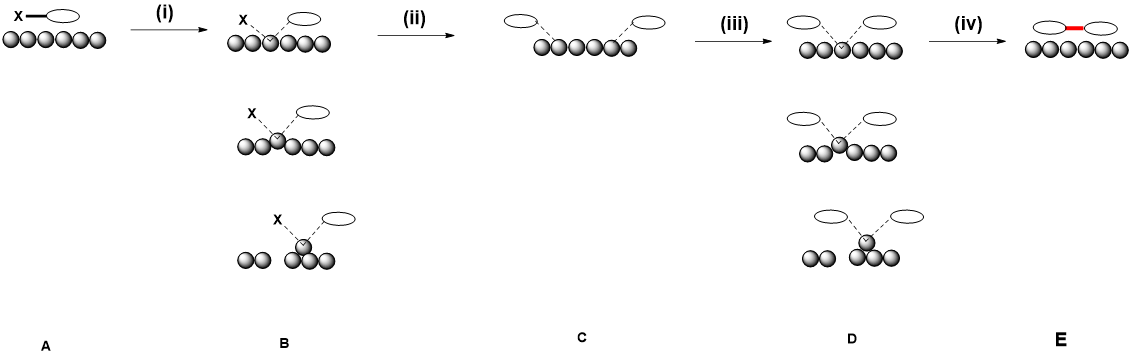
\includegraphics[width=0.9\textwidth]{Fig/mechanism.png}
%\caption{Schematic representation of elementary steps of a surface Ullmann coupling process. The following steps are shown: physisorption, dehalogenation, diffusion, formation of the organometallic bridge and then carbon-carbon bond. RZK0422: This figure needs significant improvement or it can be removed altogether. If we decide to keep it, use new pictograms and labels. It is unclear whether the adatom pathway should be shown.}
%\label{fig_mecha}
%\end{figure*}

}%end lock

%\subsection{Role of adatoms in the surface Ullmann coupling} 

{\lock

Metal surfaces are not perfect, well-ordered structures. Even single-crystal metal surfaces are not free of defects ranging from three-dimensional defect such as pores~\cite{ullmann_72} and cracks~\cite{ullmann_73} to planar defects such as twin boundaries~\cite{ullmann_74} and stacking faults~\cite{ullmann_75}, line defects such as dislocations~\cite{Ullmann_76} and to point defects such as adatoms~\cite{Ullmann_77} and vacancies~\cite{ullmann_78}.
%RZK0507: restore the figure after the sentence if Dima insists (Fig.~\ref{cyrstal_surface}).

In the process of Ullmann coupling, reactants, intermediates and final products interact directly with metal atoms on the surface and, therefore, can be affected by surface defects. 
In fact, there is a growing body of evidence that adatoms can even be created during the reaction. 
Quantifying the extent to which adatoms and other imperfections of the metal surface influence the thermodynamics and kinetics of the Ullmann coupling can suggest new strategies for surface optimization, leading, in turn, to better defect-free assembly of two-dimensional polymers. 

%RZK0426: This figure appears in wikipedia. It is relatively simple and represents ``general knowledge''. I suggest removing it from the first article and perhaps also from the review.
%\begin{figure}[htb]
%\centering
%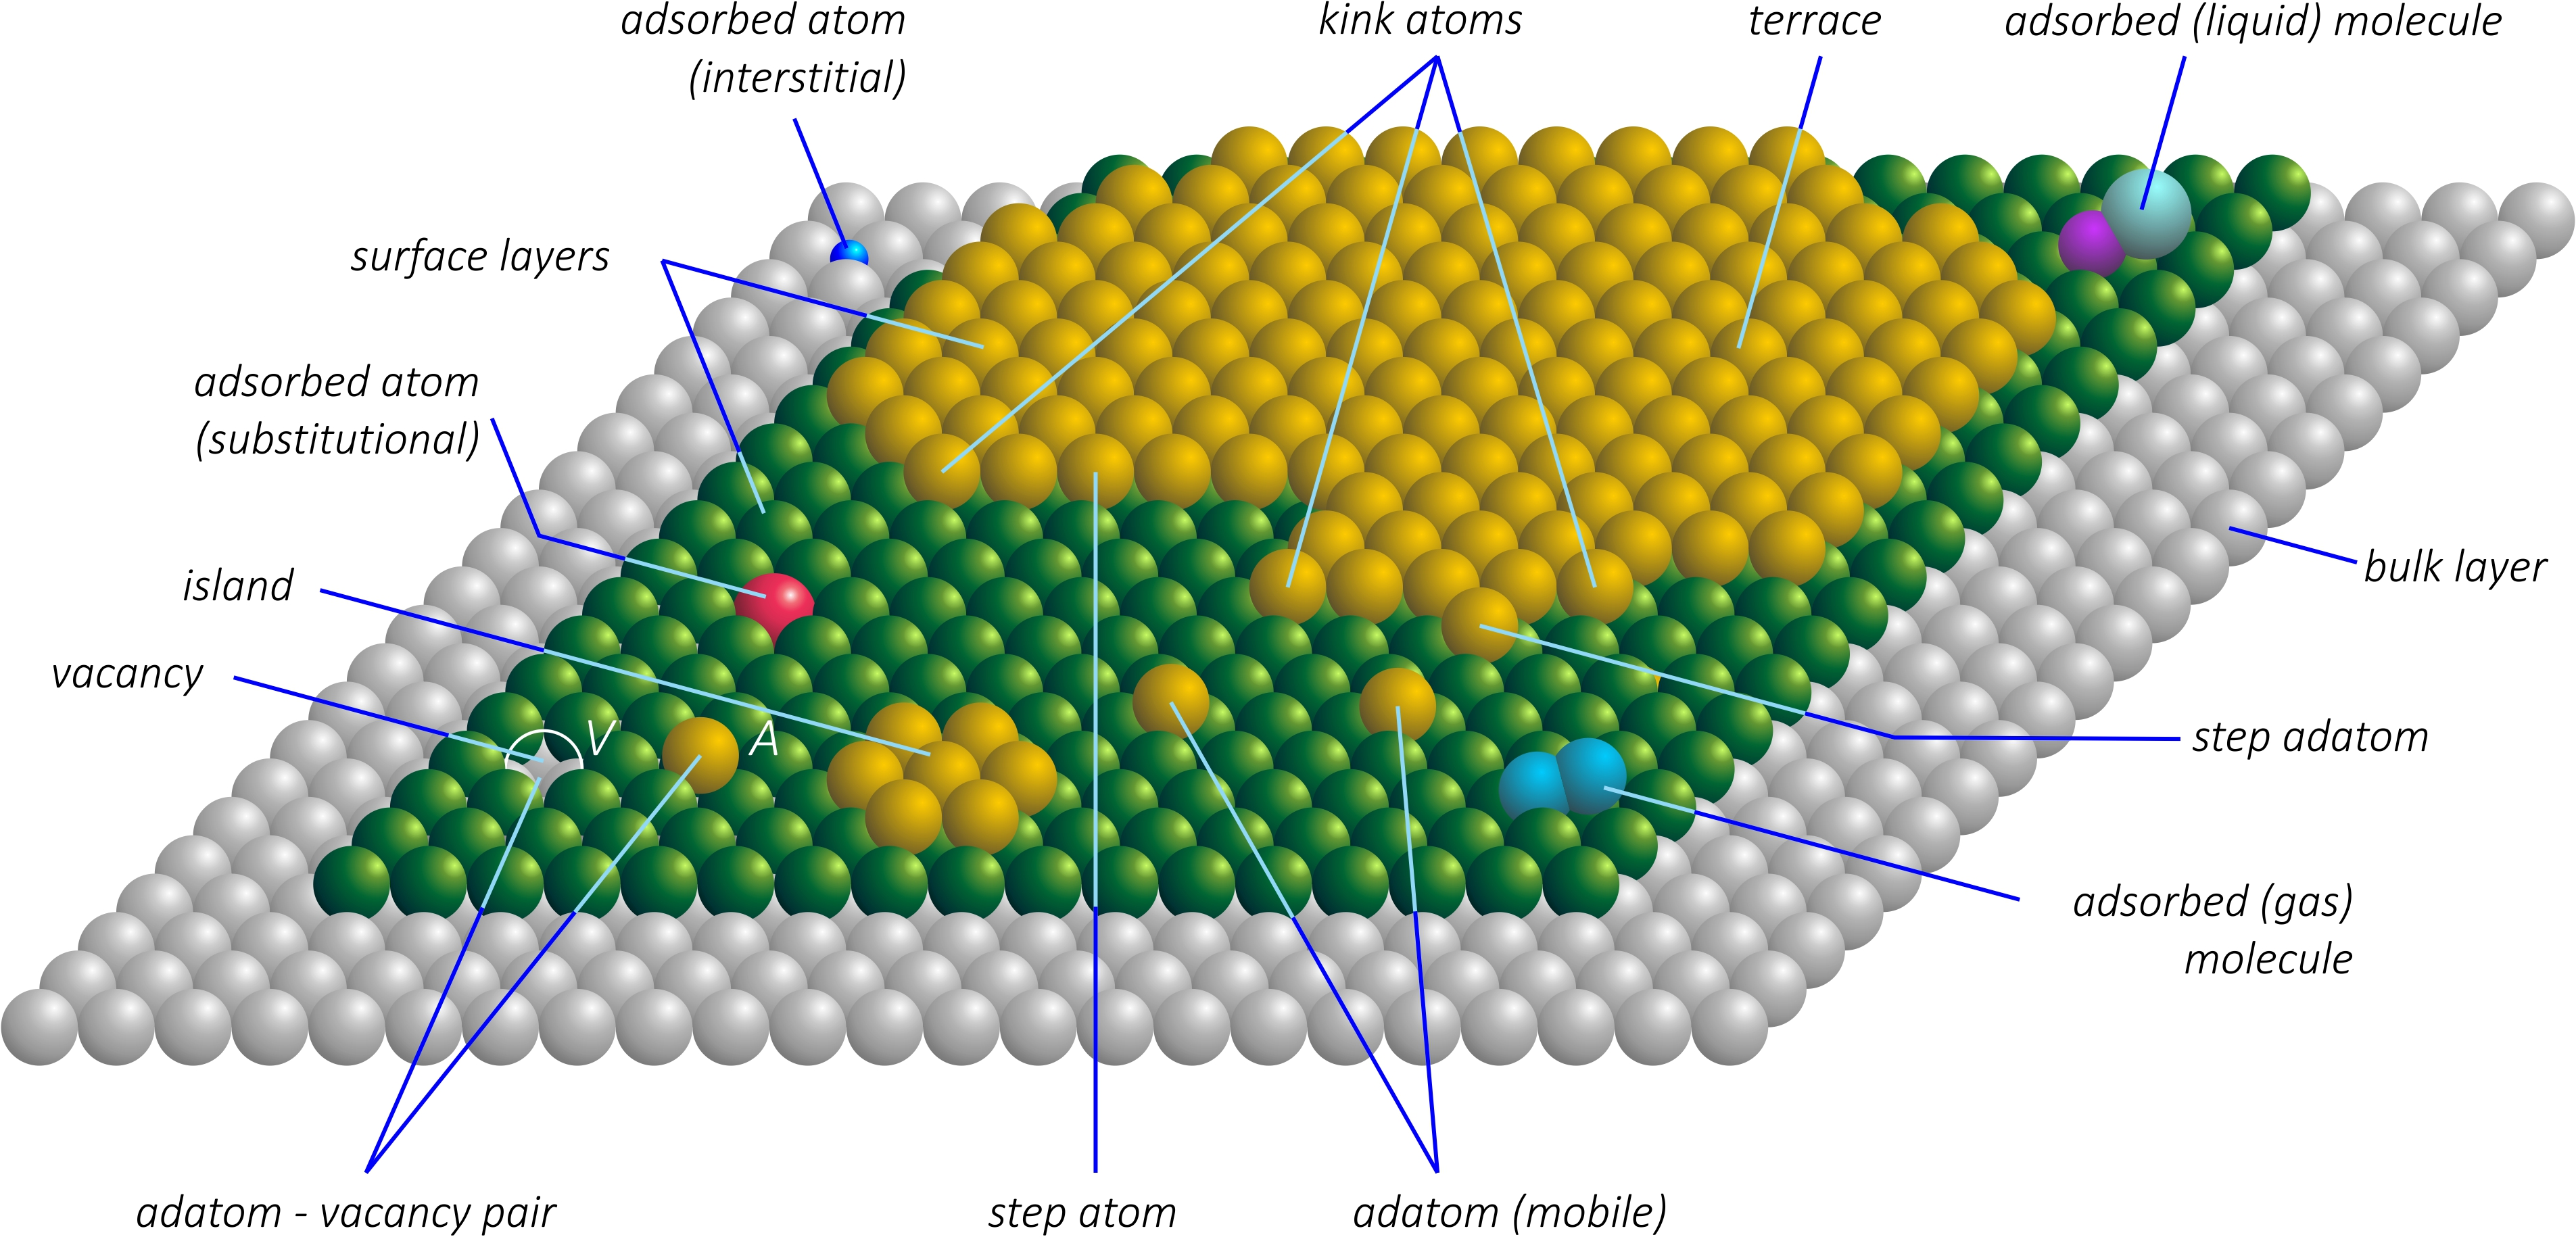
\includegraphics[width=0.4\textwidth]{Fig/Crystal_surface.jpg}
%\caption{A model of crystal surface. Adapted from Ref.~\onlinecite{ullmann_49}.}
%%RZK1221: Ignore at the moment. Remove the figure or find/create better figure. The text is almost invisible in this figure. 
%\label{cyrstal_surface}
%\end{figure}

%Surface metal atoms that affect and participate in the Ullmann coupling have different \emph{nature} and \emph{origins}.
%Atom's nature describes its immediate environment. 
To formalize discussion of the nature of surface atoms, metal atoms located within the first layer of atoms of the ideal surface will be referred to as \emph{ideal-surface} atoms. In contrast, \emph{adatoms}, according to the commonly accepted definition, lie on top of the layer of ideal-surface atoms. In this work, adatoms are differentiated according to their origin into \emph{pre-existing} and \emph{extracted} adatoms. %The origin of pre-existing atoms is irrelevant, not specified, or not known. 
Extracted adatoms are known to have been lifted from their lattice sites and placed on top of the surface leaving a surface vacancy behind~\cite{ullmann_96}. Here, \emph{vacancy} refers exclusively to vacant lattice positions on the surface, not in the bulk.

%The nature of metal atoms and the origin of adatoms have been explored experimentally and computationally.
%For origin(1), it has been reported that the onset of the vacancy-adatom formation take place on Cu(111) surface was around 900 K by molecular dynamics~\cite{ullmann_50} , which is much higher than the temperature required by surface Ullmann coupling reaction, as shown in Fig.~\ref{fig:2Dgasn}~\cite{ullmann_50}. This could be the evidence that there would not be new adatoms formation due to the thermal fluctuations as the surface Ullmann coupling proceeds. 

It is well known that Cu adatoms are created on clean Cu(111) surface by thermal fluctuations~\cite{ullmann_79, ullmann_58}. Silver and gold adatoms can be also be created especially near {\comm line, planar?} defects such as {\comm step edges, kinks?}~\cite{ullmann_84, ullmann_85}. 
It has been calculated~\cite{chemeurope2017} that the formation of an adatom on clean Cu(111), Ag(111) and Au(111) surfaces requires substantial energy of \SI{1.71}{\electronvolt}, \SI{1.12}{\electronvolt} and \SI{1.15}{\electronvolt}, respectively, making the equilibrium concentration of adatoms on clean surfaces negligibly small.  
%{\comm RZK0426: Dima's comment: ``What is known about concentration of ad-atoms on various single-crystal surfaces at RT?'' RZK agrees that stating this number is desirable. ZZ: ``I did not find it with a long time, will finish it later.''}%
Pre-exisiting adatoms have previously been observed to participate in metal organic coordination networks~\cite{ullmann_80, ullmann_81, ullmann_82, ullmann_83}, which suggests that they can play an important role in on-surface Ullmann coupling.

%\begin{figure}[ht]
%\centering
%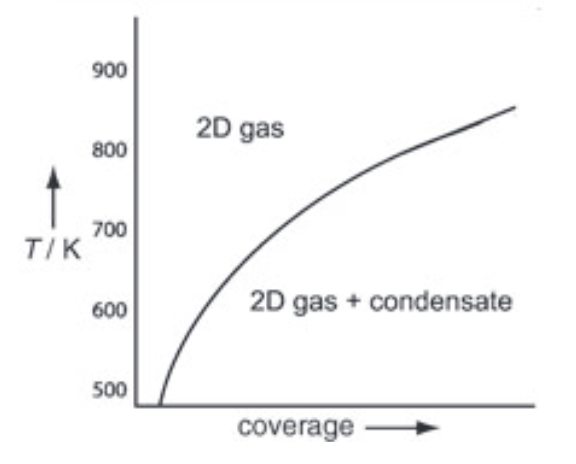
\includegraphics[width=0.75\columnwidth]{Fig/2D-gas.png}
%\caption{Schematic diagram of 2D adatom gas phase and condensed phase (islands) %coexisting at elevated temperatures for metal-on-metal systems.}
%\label{fig:2Dgas}
%\end{figure}

}

\ifdefined\INTERNAL

\subsubsection{Dehalogenation}

\begin{figure}[htb]
\centering
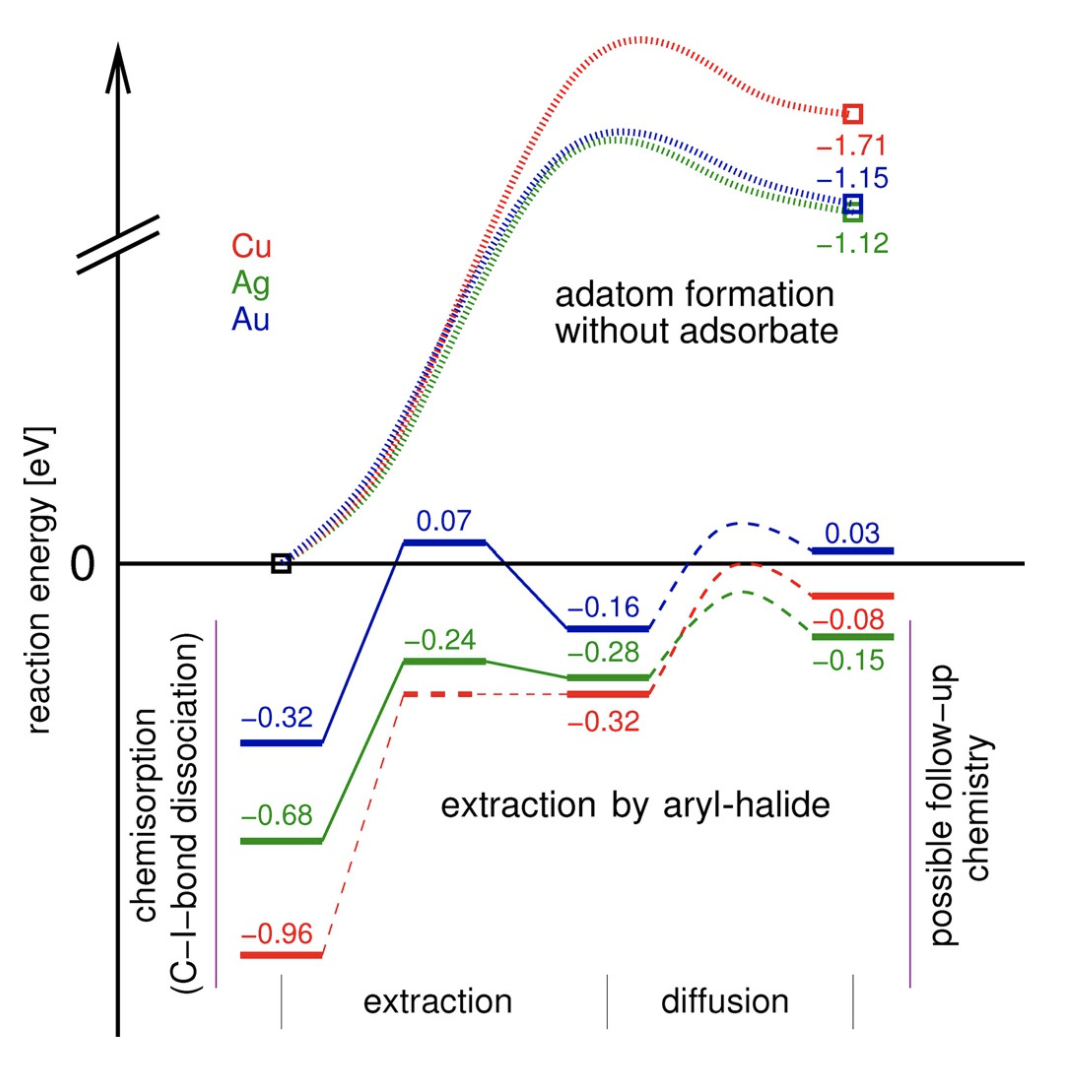
\includegraphics[width=0.75\columnwidth]{Fig/Adatom-formation.png}
\caption{Graphical comparison of the energetics of the adatom formation without adsorbate (top half) to the extraction by aryl–halide process (lower half).Values for Cu are shown in red, for Ag in green and for Au in blue. The extraction-by-arylhalide process starts from the dissociated iodobenzene. Dotted lines indicate parts of the energy profile that have not been quantitatively resolved. Adapted from Ref.~\cite{chemeurope2017}}
\label{fig:3}
\end{figure}

\fi

{\lock

It has been suggested based on results of STM investigation and DFT calculations that adatoms can be created immediately after the dehalogenation of aryl precursors in the on-surface Ullmann reaction. 
%REVIEW: As shown in Fig.~\ref{fig:3}, 
The calculated energy required to lift an ideal-surface atom and place it on the surface is reduced to \SI{0.64}{\electronvolt}, \SI{0.40}{\electronvolt} and \SI{0.16}{\electronvolt} for Cu(111), Ag(111) and Au(111) surfaces, respectively, if the extracted adatom is bonded to iodine and phenyl fragments -- the products of the dehalogenation of a iodobenzene molecule~\cite{chemeurope2017}. {\comm RZK0506: The energy for Cu appears to be wrong. Discuss the energies with me.}
%
It has also been concluded that the significantly reduced adatom extraction energy (compared to that on the clean surface) can be fully compensated by the release of comparable amount of energy in the preceding dehalogenation step, making the combined dehalogenation and extraction essentially thermo-neutral on these surfaces.

%RZK: For future comparison in RnD: extraction here is still hugely endothermic, unlike the extraction at later steps.

}

\ifdefined\INTERNAL

\subsubsection{Diffusion}

%\begin{figure}[hbt]
%\centering
%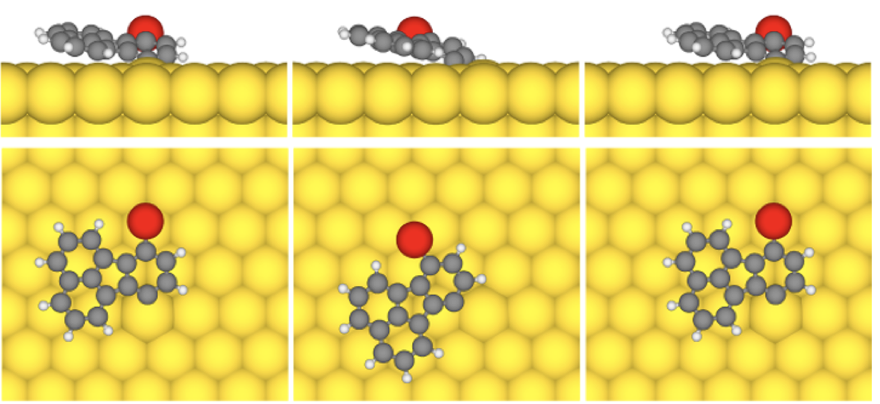
\includegraphics[width=0.75\columnwidth]{Fig/Diffusion_path.png}
%\caption{Top and side view of the initial, transition and final geometries of bromofluoranthene molecule diffuse. Adapted from Ref.~\cite{jpcc2018}}
%\label{fig:diff}
%\end{figure}

\fi

{\lock

Little effort has been dedicated to exploring the possibility of the adatom extraction during the diffusion of the dehalogenation products  -- single organic molecules and halogens -- on an ideal metal surface. 
%
%No evidence has been reported that the products of the dehalogenation -- single organic molecules and halogens -- can extract adatoms while diffusing on an ideal metal surface. 
%
It has been calculated that a single phenyl group diffusing on Cu(111) lifts a copper atom only by \SI{0.16}{\angstrom} from its original position~\cite{pccp2010}. 
This raise is considered insufficient to justify further studies of the adatom creation.
However, larger organic groups that tend to stay parallel to the surface can lift a metal atom higher. 
For example, DFT calculations have revealed that bromofluoranthene group, which contains four fused aromatic rings, lifts a gold atom by \SI{0.5}{\angstrom} above its ideal-surface position~\cite{jpcc2018} in the optimized state. 
Moreover, it has been calculated that this radical can lift the gold atom upto \SI{1.9}{\angstrom} in one of the intermediate NEB states in the diffusion pathway~\cite{jpcc2018}.
The raise of this magnitude (cf. \SI{1.7}{\angstrom} van der Waals radius of gold atom) is high enough to warrant further exploratory studies.

%RZK0511: The following paragraph does not seem to belong in the literature review. If these are your own thoughts then the paragraph should be placed in R&D. If this is a summary of someone else' review of existing data then it should be properly referenced.
%The evidence of pre-existing adatoms are involved in this step is not reported. It can be speculated that diffusion of aryl groups on metal surface can seldom create adatoms since the intensity of interaction between one dehalogenated species and metal atoms is not sufficient to fully extract ideal-surface atoms out.

}

\ifdefined\INTERNAL

\subsubsection{Formation of carbon-metal-carbon intermediates} \label{sec:dimerized-adatom}

\begin{figure}[tb]
\centering
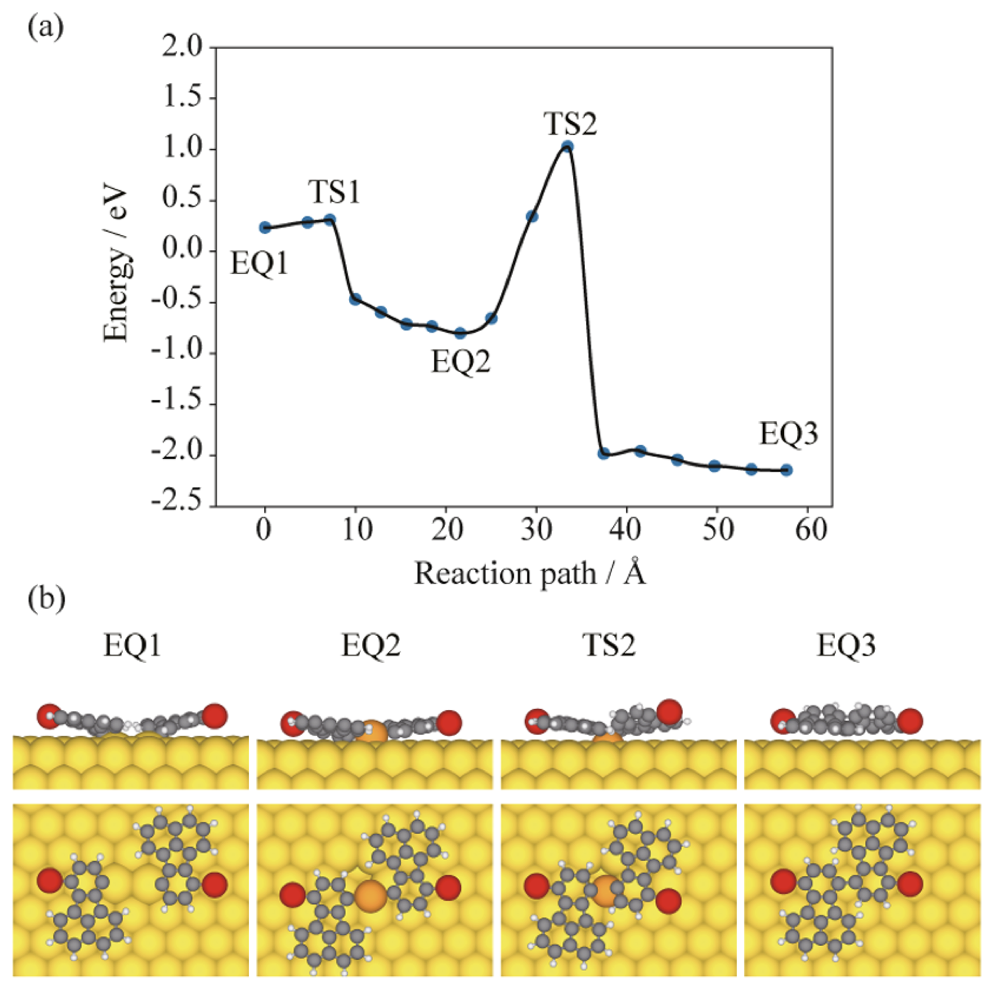
\includegraphics[width=0.75\columnwidth]{Fig/adatominformation.png}
\caption{(a) Energy profile of the coupling reaction of bromofluoranthene radicals through an organometallic intermediate along the reaction path. The horizontal axis indicates the distance between neighboring images. The energy is shown with respect to that of an isolated radical on the surface. (b) Top and side views of the initial (EQ1), transition (TS1, TS), intermediate (EQ2), and final (EQ3) geometries. Adapted from Ref.~\cite{jpcc2018}}
\label{fig:high-lift}
\end{figure}

\begin{figure}[bt]
\centering
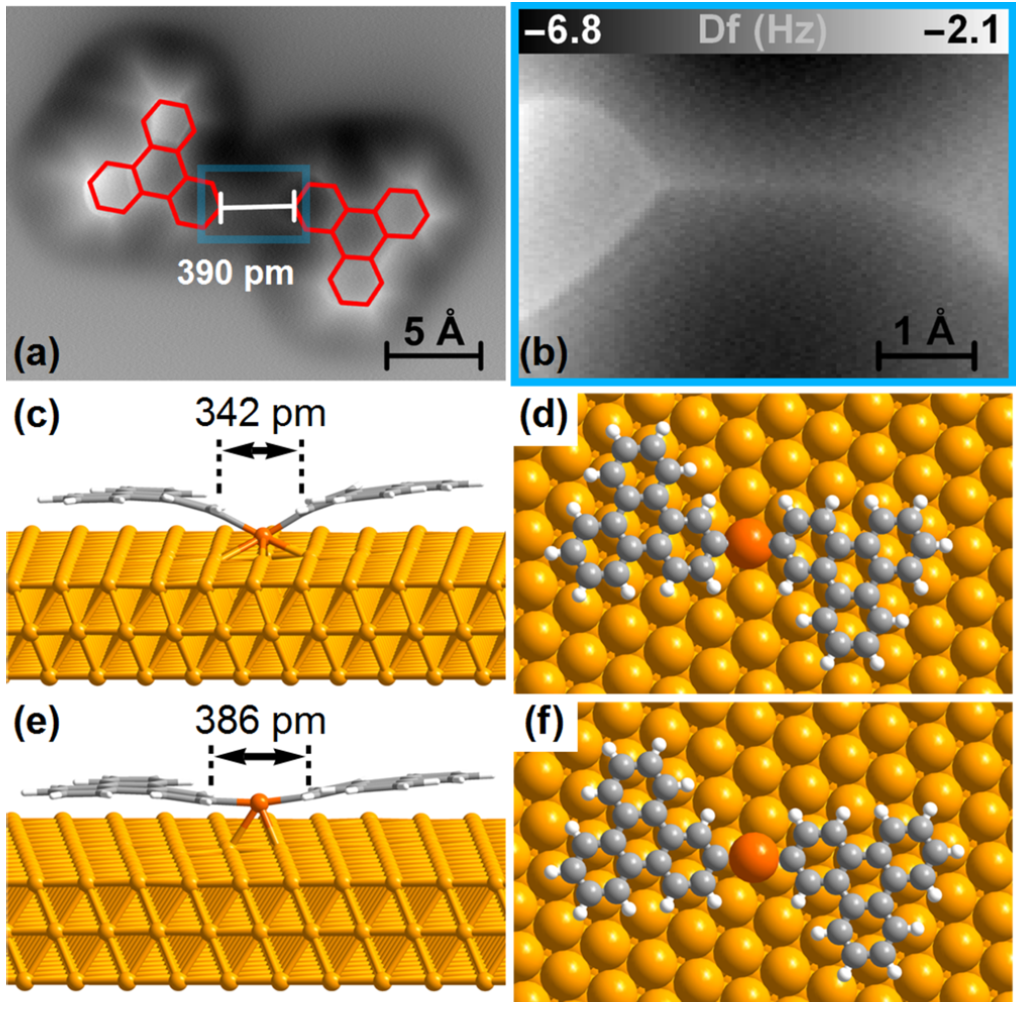
\includegraphics[width=0.75\columnwidth]{Fig/distance.png}
\caption{(a) AFM frequency shift image of intermediate with fit of structural model. (b) Zoom on intermediate bond ($cf$. blue box in a) imaged with decreased tip-sample distance ($\Delta$z = -70 pm with respect to image a). (c--f) DFT-D3 calculations [PBE-D3/ pw (PAW P)] for two different organometallic intermediate states (surface atom (c,d) vs adatom (e,f)). Adapted from Ref.~\cite{acsnano2017}}
\label{fig:adatom-CMC-evidence1}
\end{figure}

\begin{figure}[tb]
\centering
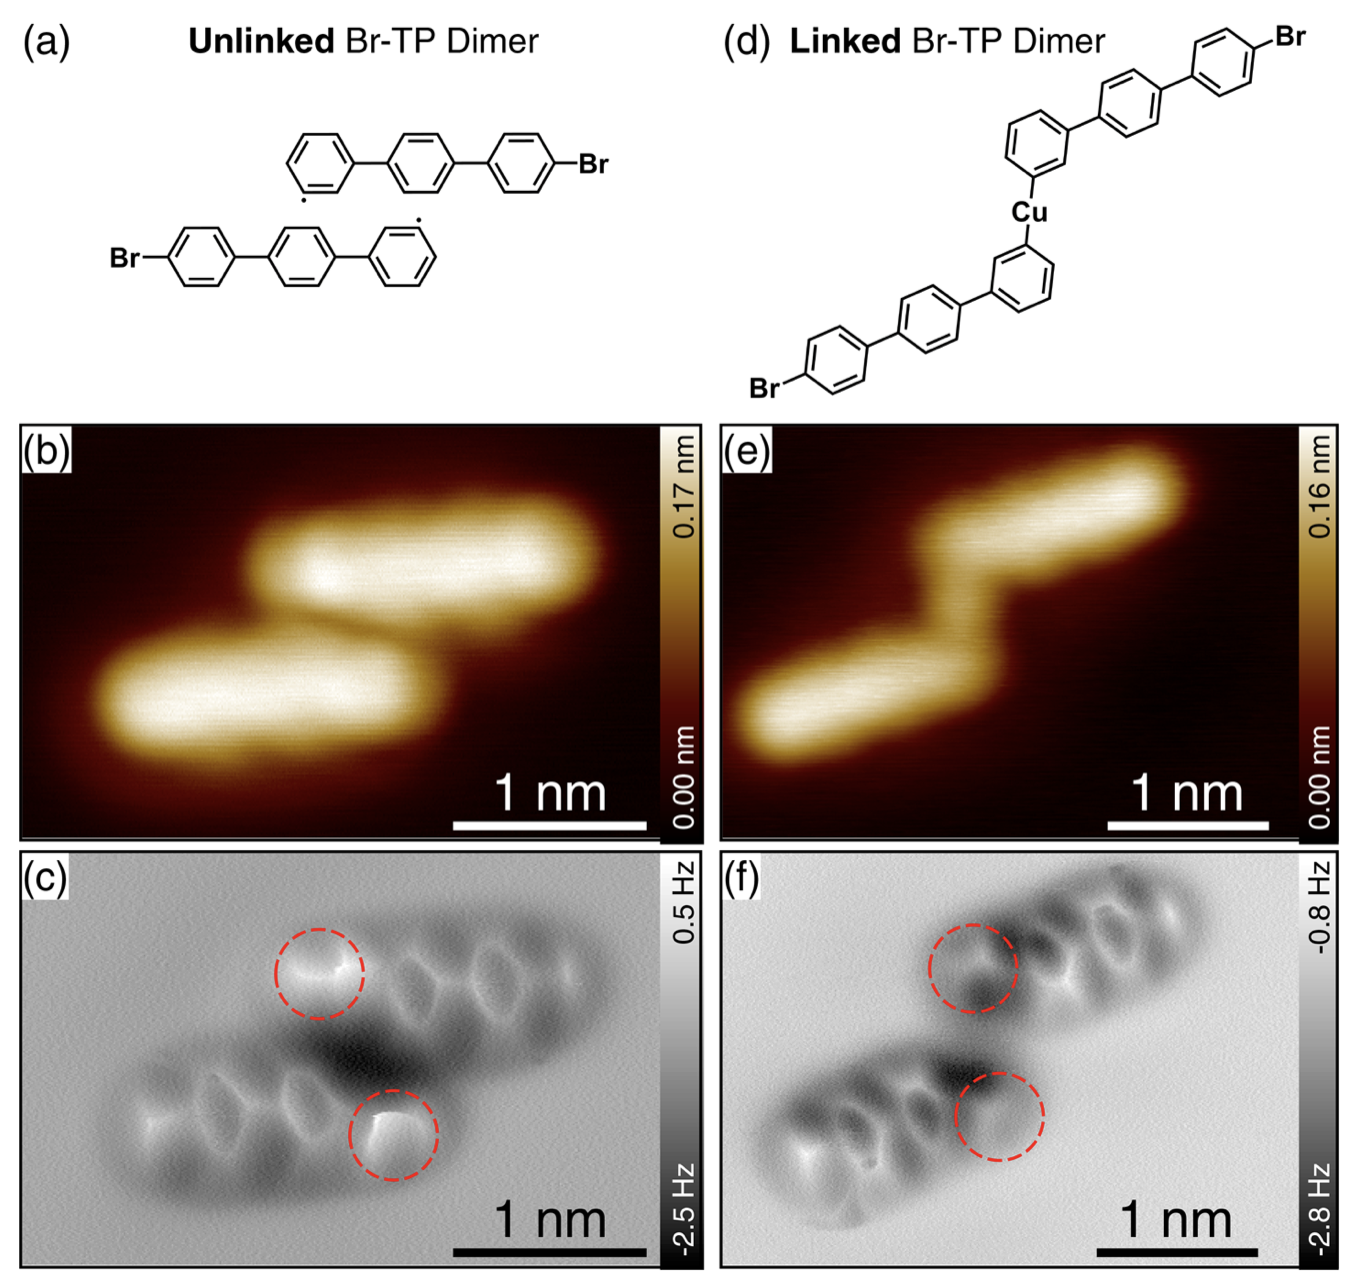
\includegraphics[width=0.75\columnwidth]{Fig/AFM_prove.png}
\caption{Molecular structures (top row), STM (middle row), and AFM images (bottom row) of 4‐Bromoterphenyl dimers on Cu(111). Two different types of dimers are observed, which are denoted as unlinked (left column) and linked dimers (right column). The STM image of the unlinked dimer reveals a dark region between the two molecules that separates them. Between the two molecules of the linked dimer a bright protrusion is observed in the STM scan that directly links them. The red dashed circles in (c) and (f) indicate the twisted phenyl rings, which lost their iodine atoms. Imaging parameters: (b) 200 mV, 30 pA, (e) 200 mV, 10 pA, tip height z = -100 pm (c) and z = -24 pm (f) with respect to a tunneling set point of 200 mV and 10 pA on Cu(111). Adapted from Ref.~\cite{acsnano2019}}
\label{fig:adatom-CMC-evidence2}
\end{figure}

\fi

%%In addition, chlorinated prophyrin as precursor has also been deposited on Cu(111)~\cite{chematerial2019}. Based on DFT calculations, the Cu adatom mediated path is 3~eV lower than the direct dechlorination. And from STM image, some precursors are still intact at temperature of 400~K, which should be already dehalogenated at lower temperature. It proves that the Cu adatoms are the limiting agent [Fig.~\ref{fig:prophyrin}].

%\begin{figure}[ht]
%\centering
%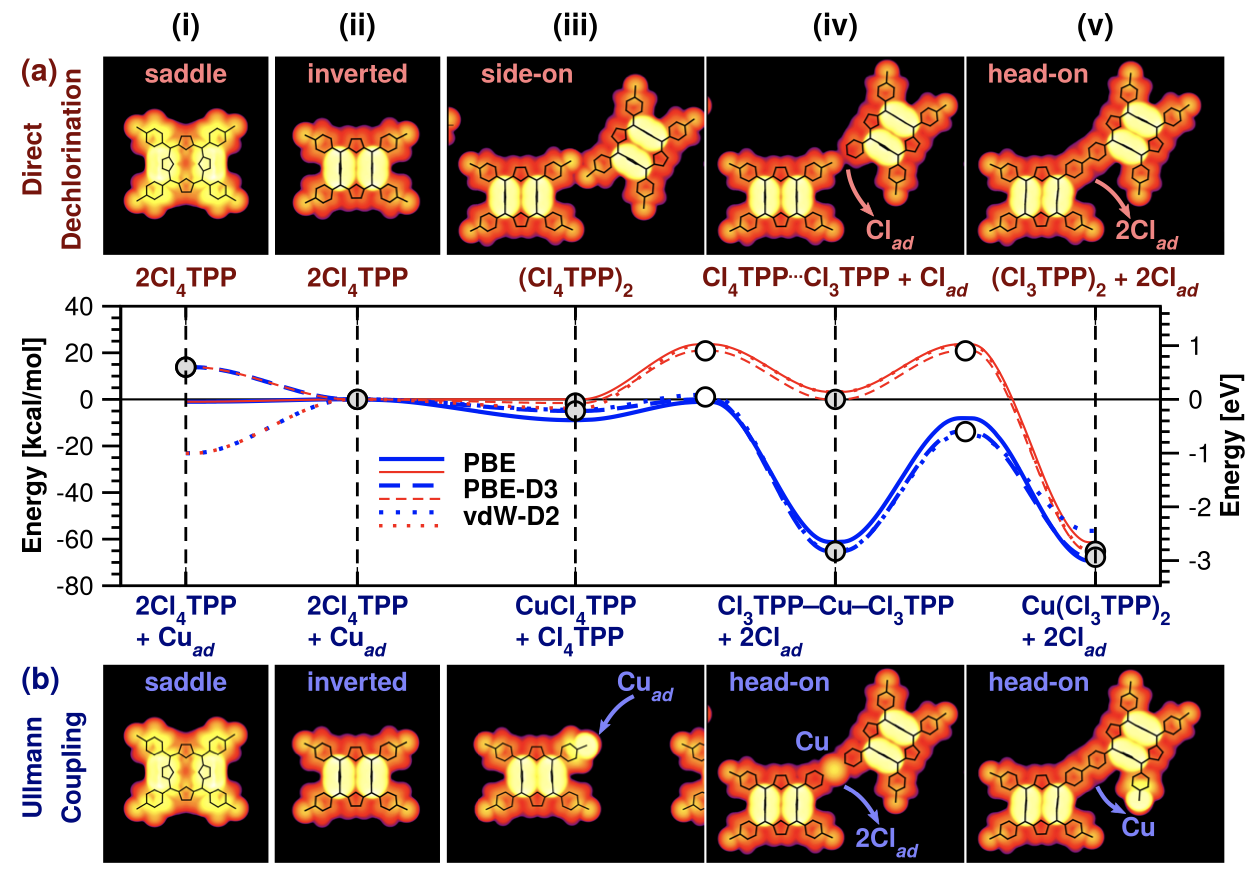
\includegraphics[width=0.4\textwidth]{Fig/Complete.png}
%\caption{STM simulations and DFT reaction profile for the (a) direct %dechlorination reaction (red lines) and (b) Cu adatom-mediated Ullmann coupling reaction (blue lines). For each process the energy are plotted of the (i, ii) precursors, (iii, iv) intermediates, (v) and final species (gray circles) and two transition states (white circles).}
%\label{fig:prophyrin}
%\end{figure}

{\lock

In contrast to the diffusion step, the role of adatoms in the formation of carbon-metal-carbon bridge structures has been investigated previously~\cite{acsnano2017, acsnano2019}. %RZK0518: Should we also cite adatom-related works referenced in acsnano2017? I do not think they are Ullmann related but they seem to consider the adatom question. Additionally, the following excerpt from acsnano2019 indicates that the role of adatomshave been studied more extensively than ZZ reports here. ``In the literature cases are reported where dehalogenated molecules are bound either to metal surface atoms or to adatoms, and there is a current debate about this topic.10,48,52−59,77''
The attention to adatoms in this step stems from the realization that the force exerted upon a metal atom by two aryl radicals might be sufficiently strong to lift it high above its ideal-surface position and to make its diffusion away from the vacancy plausible. 
For example, DFT modeling shows that two bromofluoranthene groups lift their shared gold atom \SI{2.2}{\angstrom} above its ideal surface position, which is noticeably higher than the \SI{0.5}{\angstrom} raise produced by a single group~\cite{jpcc2018} and than the radius of the metal atom.
%REVIEW (Fig.~\ref{fig:high-lift}). 
%{\comm RZK0518: It is perhaps worth mentioning (here or later) that, while this is not a fully extracted adatom, it is shifted to the side of its original position, leaving something that looks like a vacancy behind. This distinction is very important to draw a clear ditinction between highly-lifted surface atoms and adatoms.}

The participation of an adatom in the formation of the C--M--C bridge has been considered explicitly in the case of intermediates formed by two triphenylene groups on Cu(111) surface. 
%REVIEW (Fig.~\ref{fig:adatom-CMC-evidence1}). 
The \SI{3.90\pm 0.25}{\angstrom} carbon-carbon distance measured using AFM has been found to agree more closely with the \SI{3.86}{\angstrom} distance calculated for a DFT model with an adatom acting as the bridge rather than with \SI{3.42}{\angstrom} distance calculated for the model with a highly lifted ideal surface atom~\cite{acsnano2017}. 
The close agreement between the measured distance and the former model has been interpreted as evidence of the adatom participation in the Ullmann coupling of bromotriphenylene molecules on Cu(111) surface. 
%
The structural analysis has been supported by the analysis of the energetics of the formation of the C--M--C intermediate from two chemisorbed dehalogenated groups and a pre-existing adatom on Cu(111). This energy has been found to be \SI{1.74}{\electronvolt} lower than the energy of the formation of the intermediate on the ideal surface~\cite{acsnano2017}. It should be noted, however, that the large amount of energy required to create the adatom has not been taken into consideration in this work.

%Fig.~\ref{fig:adatom-CMC-evidence1} describes the C--Cu--C structure formed by two triphenylene moieties with a copper atom on Cu(111) surface using AFM and DFT methods~\cite{acsnano2017}. Two distinct simulation models are shown: (1) the copper atom in C--Cu--C structure comes from ideal surface atom as shown in (c) and (d). This ideal surface atom is partially lifted up from its original position in the first layer of metal; and (2) the copper atom in C--Cu--C is an adatom as pictured in (e) and (f). Two model are compared with AFM image on atomic properties. The distance between carbon and carbon in this C--Cu--C bridge in AFM, ideal surface model and adatom model are \SI{3.90}{\angstrom},  respectively, which shows that the adatom model is more consistent with the molecule geometry in experiment. This is in agreement with DFT calculations showing that the energy for formation of C--Cu--C bridge structure from these precursors with adatom is estimated to be \SI{1.74}{\electronvolt} lower than with ideal surface atom, both from two chemisorbed dehalogenated radicals on Cu(111) surface as initial states. %This proves that it is likely to be adatom that make up the C--M--C structure.

A comparison of the twisting angle in experimental and simulated AFM images of the C--M--C intermediates formed by two 4‐bromoterphenyl groups on Cu(111) surface 
%REVIEW (Fig.~\ref{fig:adatom-CMC-evidence2}) 
has also confirmed that it is an adatom that serves as the metal bridge~\cite{acsnano2019}. Furthermore, an analysis of the temperature-dependent ratio of the two types of C--M--C intermediates that are observed for this precursor has led to conclusion that the bridge adatoms are extracted during the C--M--C formation step of the surface Ullmann coupling reaction, not simply present on the clean surface before the reaction~\cite{acsnano2019}. 
%REVIEW: {\comm RZK0518: The figure shown is insufficient to clarify the text. Discuss: either use the other figure from the manuscript or combine or remove figures altogether.}

}

%RZK0426: Has the statement below from jacs2013 been incorporated? 
%Furthermore, the presence of Cu adatoms may impact the self-assembly more than the poor diffusion on the atomically flat Cu(111) surface. These adatoms are known to have a great influence on selfassembly on Cu(111), where in many cases coordination bonds are formed instead of covalent networks.21 The Cu adatoms can also contribute to the covalent bonding of the nanostructure.22,23 (%ZZ maybe we should add this in the diffusion section in adatom part)

%\subsubsection{Formation of the carbon-carbon bond}

{\lock

The role of adatoms in the formation of the carbon-carbon bond, the final key step of the on-surface Ullmann coupling, has not been investigated. Although the C--C bond formation on a gold atom lifted high above the surface has been studied computationally in the case of bromofluoranthene,
%REVIEW: (Fig.~\ref{fig:high-lift}), 
the investigation focused exclusively on the pathway where the lifted atom returns to its original crystallographic position in the surface~\cite{jpcc2018}. 

}

\ifdefined\INTERNAL

\subsection{Open questions}

\fi
%OPEN QUESTIONS
{\lock

Despite the evidence of adatoms being a part of some organometallic bridge structures~\cite{acsnano2017, acsnano2019}, it remains unclear whether surface atoms can be extracted by two organic groups and what groups are more likely to extract adatoms. Moreover, it is unknown whether the extracted adatoms can be left behind on the surface, uncoordinated to any groups, after the completion of the carbon-carbon bond formation to participate in other catalytic steps of the Ullmann coupling.

%SHORTER VERSION: It remains unclear whether surface atoms can be completely extracted by two organic groups and, after the completion of the carbon-carbon bond formation, be left behind on the surface to affect other reacting species. %in subsequent catalytic cycles of the Ullmann process.
%ANOTHER VERSION: It remains unclear whether two organic groups can extract an adatom, which, after the completion of the carbon-carbon bond formation, is left behind on the surface to participate in subsequent catalytic cycles of the Ullmann process.

}

\ifdefined\INTERNAL

\subsection{Objectives}

\fi

{\lock

In order to answer these questions, the energetics of the adatom creation during the Ullmann reaction of two phenyl groups on Cu(111) surface is examined for the first time using DFT modeling. 
More importantly, previously unstudied effects of adatoms, extracted and pre-existing, on the coupling of two phenyl groups are investigated in detail. 
The phenyl groups, which are produced in the dehalogenation of monosubstituted benzenes, are chosen in this work as the simplest and most studied representatives of aryls participating in an on-surface Ullmann reaction. Due to their small size, phenyl groups are expected to be the least likely aryls to extract adatoms on the surface.

%Can the coupling be effectively catalyzed by an adatom, extracted or pre-existing? Is the energy of the reaction sufficient to create an adatom and whether there are any barriers along the extraction pathway?

%While some studies (e.g. C-M-C bridge) have assumed the presence of adatoms, it is important to understand whether this adatoms can be created and, if yes, how (thermal fluctuations on the pure surface, which elementary steps of the Ullmann process).

%The creation of ``clean'' adatoms has not been considered previously because, in all previous studies either (a) the lifted atom returns back to the vacancy or (b) remains bound to the groups that facilitated its extraction. Furthermore, energetic considiration in C-C stages do not account for the energy required to create adatoms.

}

\section{Computational methods}

{\lock

Cu(111) surface was modeled with a $20.55 \times 13.35$~\si{\angstrom} slab containing 192 Cu atoms arranged in four 8 $\times$ 6 atomic layers. \SI{10}{\angstrom} of vacuum was added in the direction normal to the surface to ensure weak interaction between periodic images of the slab.
%RZK0602: The vacuum layer seems to be too thin.

DFT calculations were performed using Vienna \emph{ab initio} simulation package (VASP)~\cite{ullmann_131, ullmann_132, ullmann_133, ullmann_134}. The dispersion-corrected~\cite{ullmann_136, ullmann_137} Perdew-Burke-Ernzerhof (PBE) generalized gradient approximation~\cite{ullmann_139} was used as the exchange-correlation (XC) functional. 
%RZK0602: The two references above are not the correct citation for PBE.
Spin-polarized electronic states were modeled using a plane wave basis set with the energy cut-off set at \SI{800}{\electronvolt}.
%RZK0602: Why the energy cutoff is so high? {\zhzh ZZ0602: corrected}
The projector augmented wave formalism was used to describe interactions of atomic cores with valence electrons. The integration over the Brillouin zone was performed using the $3\times 3 \times1$ Monkhorst-Pack $k$-point mesh. 

Atomic positions were optimized until the maximum force on atoms decreased below \SI{0.02}{\electronvolt\per\angstrom}. 
Transition state structures were located using the climbing-image nudged elastic band (NEB) with the VTST code~\cite{ullmann_59}. 
In NEB calculations, an improved initial guess~\cite{ullmann_60, ullmann_99} for the minimum energy path was used and the positions of atoms were relaxed until the maximum force dropped below \SI{0.1}{\electronvolt\per\angstrom}.

}

\section{Results and Discussion}

\begin{figure*}[hbt]
\centering
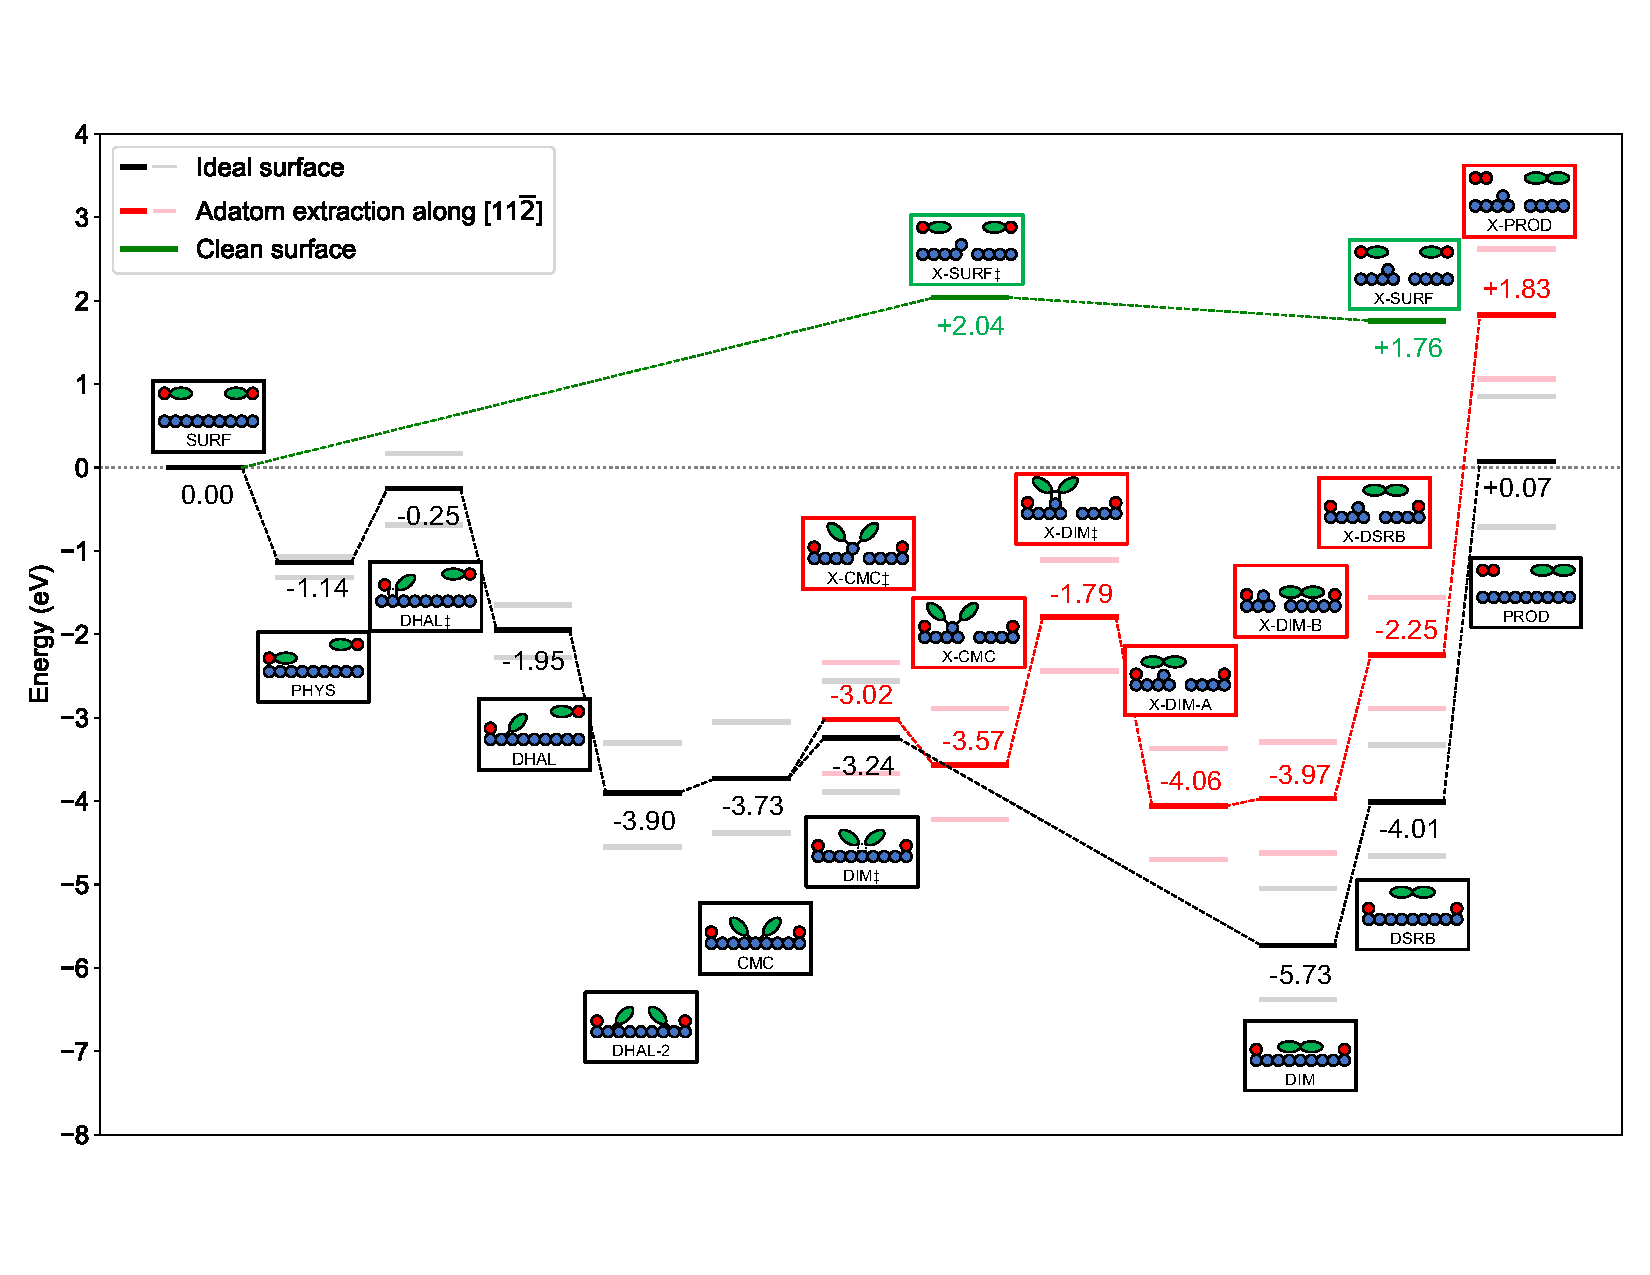
\includegraphics[width=1.\textwidth]{Fig/main-profile.pdf}
\caption{Energy profile of the Ullmann reaction of monohalogentated benzenes on the Cu(111) surface. In the schematic labels, blue and red circles denote copper and halogen atoms, respectively, whereas green ovals denote phenyl groups. Levels shown with bright colors are states with bromine as the halogen, whereas the faint upper and lower levels denote states with chlorine and iodine as the halogen, respectively. The energy of the ideal metal surface and two gas-phase monohalogenated benzene molecules, denoted here as \textbf{SURF}, was used as the zero-energy reference. The energy of the chlorine and iodine containing species are reported in Tables~\ref{SI-table:bondlength}, \ref{table:idealsurface} and~\ref{table:adatom-longitude}.
 {\comm RZK0603: Use the same font, same size for all labels: energy levels, axis ticks, axis labels. The energy levels numbers are poorly aligned and make the figure look bad. Do not insert energy labels manually, add them with your plotting tool.} {\zhzh ZZ: modified}
}
\label{fig:completeenergy}
\end{figure*}

\ifdefined\INTERNAL
\subsection{Physisorption}
\fi

{\lock

\textbf{Early steps of the Ullmann process.} Organic precursors are physisorbed on a metal surface before undergoing chemical transformations. 
Although the binding of chlorobenzene, bromobenzene and iodobenzene to Cu(111) calculated in this work (Fig.~\ref{fig:completeenergy}, \textbf{PHYS} state) is stronger than that obtained previously using the a different XC functional~\cite{jacs2013} the trends in the physisorption energies for different halogens are almost exactly the same (Table~\ref{SI-table:bondlength} in \sinfo).
%REVIEW: The strong binding between the surface and halogenated benzenes is primarily due to the interaction of (a) the $\pi$-system (b) halogen (choose one) and the surface. This follows from the analysis of the interaction energy between biphenyl and the metal (\SI{1.72}{\electronvolt}) and the van derWaals interaction of Br$_2$ molecule with the surface (\SI{1000}{\electronvolts}).
}

\ifdefined\INTERNAL
\subsection{Dehalogenation}
\fi

\begin{figure*}[hbt]
\centering
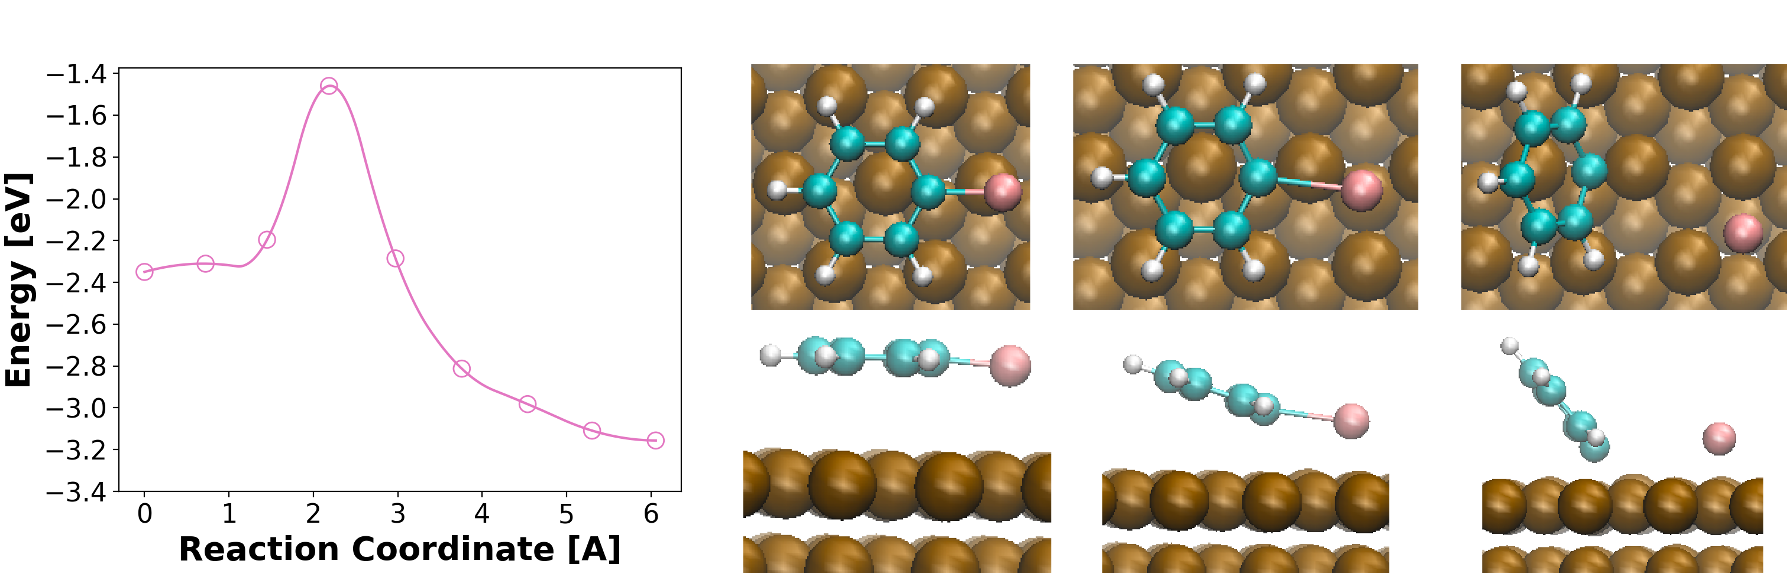
\includegraphics[width=1.0\textwidth]{Fig/dissociation_Br.pdf}
\caption{Dissociation of the C--Br bond on Cu(111) surface. The energy diagram shows the NEB profile of the debromination process. In the structural images, yellow, cyan, white, red spheres represent copper, carbon, hydrogen, bromine atoms, respectively. The dissociation of the C--Cl and C--I bonds is shown in \sinfo.
{\comm RZK0603: Top-side views are poorly aligned, spacing between the state figures are different, the white margin on top the figure is too large. It is time to start polishing figures and tables in \sinfo using the same standards as in the main text. }
}
\label{fig:dissociation_Br}
\end{figure*}

{\lock

Fig.~\ref{fig:dissociation_Br} shows the structures of the initial, transition and final states for the debromination of the physisorbed bromobenzene on Cu(111). These states are labeled as \textbf{PHYS}, \textbf{DHAL$\ddagger$} and \textbf{DHAL}, respectively. Chlorobenzene and iodobenzene undergo similar structural transformation during the dehalogenation step (Figs.~\ref{SI-fig:dissociation_Cl} and~\ref{SI-fig:dissociation_I} in \sinfo).
%
%REVIEW (Numbers should be verified): Unlike analogous reactions in the solution, dehalogenation reactions on the copper surface are all exothermic. DFT results have demonstrated that the energy barrier of nucleophilic substitution of chlorobenzene and bromobenzene in solution are \SI{1.11}{\electronvolt} and \SI{1.18}{\electronvolt}~\cite{ullmann_86}.
%
The energy barrier of the dehalogenation on Cu(111) surface decreases from chlorobenzene (\SI{1.25}{\electronvolt}) to bromobenzene (\SI{0.92}{\electronvolt}) and to iodobenzene (\SI{0.68}{\electronvolt}). 
The amount of energy released in the dehalogenation follow the opposite trend increasing from chlorobenzene (\SI{0.58}{\electronvolt}) to bromobenzene (\SI{0.80}{\electronvolt}) and to iodobenzene (\SI{0.94}{\electronvolt}) (Fig.~\ref{fig:completeenergy} and Table~\ref{SI-table:bondlength} in \sinfo), in accord with the Bell-Evans-Polanyi principle.
%
The calculated energies are in qualitative agreement with the trend in experimentally measured dehalogenation temperatures~\cite{ullmann_52,ullmann_87,ullmann_67} and with the previous calculations on this~\cite{jacs2013} and similar systems.
%{\comm RZK0527: REVIEW only becuase the trend is reproduced only roughly. On Cu(111), iodobenzene has been observed to dissociate at \SI{175}{\kelvin}~\cite{ullmann_87} while bromobenzene dissociates at \SI{160}{\kelvin}~\cite{ullmann_67}. There is no data the dehalogenation temperature of chlorobenzene, but it can be inferred from the existing data on dihalogenated precursors (Table~\ref{table:exp-temp}) that chlorobenzene dissociates at significantly higher temperature than both bromobenzene and iodobenzene.}

%REVIEW: It should be noted that the dehalogenation of bromobenzene and iodobenzene on Cu(111) has been investigated previously~\cite{jacs2013} using optB86b exchange-correlation functional and smaller slab size, the molecular orientation on Cu(111) is identical with our model. The previous energy barrirer of this step are \SI{0.66}{\electronvolt} (bromobenzene), \SI{0.44}{\electronvolt} (iodobenzene). The previous energy change is \SI{-0.68}{\electronvolt} (bromobenzene) and \SI{-0.81}{\electronvolt} (iodobenzene). The slight difference in the energy value can be interpreted by different functional usage and our larger slab model for computation.

%RZK0527: The following paragraph discusses details that are not relevant to the current topic. It is commented out and can be restored when REVIEW is written.
%{\zhzh
%Selected geometric parameters of the intermediates have also been summarized in Table~\ref{table:bondlength}. 
%In \textbf{PHYS} of halobenzene, the distance between carbon and halogen is consistent with the C--halogen covalent bond length (\SI{1.76}{\angstrom} in chlorobenzene, \SI{1.91}{\angstrom} in bromobenzene and \SI{2.14}{\angstrom} in iodobenzene, respectively) in gas phase calculated based on B3LYP functional. These distances show a continued growth till \textbf{DHAL} states, and dissociated halogen atoms all occupy the hollow sites on Cu(111) surface in the end of dehalogenation. Interestingly, C--halogen distances in three different \textbf{DHAL$\ddagger$} show consistent approximately \SI{0.5}{\angstrom} longer than corresponding C--halogen lengths in \textbf{PHYS} , suggesting that different dehalogenation reactions on Cu(111) follow similar mechanisms.
%The angle of phenyl ring also suffers successively changes, parallel in \textbf{PHYS}, tilt in the process of dehalogenation and finalize with an apparent slope in \textbf{DHAL}. The interaction between unsaturated carbon and copper atom shortens their distance to same \SI{2.01}{\angstrom} in three different \textbf{DHAL} states, and these copper atoms are all raised approximately by \SI{0.12}{\angstrom} from their original positions.
%The same C--Cu distances in \textbf{DHAL} suggest that the dissociated halogen atoms have little effect on phenyl--Cu intermeidate. However, halogen atoms have obvious influence on dissociated phenyl ring, resulting in their different tilt angles, deiodinated phenyl ring is inclined around \SI{70}{\degree} to metal surface, larger than debrominated and dechlorinated phenyl rings both at around \SI{50}{\degree}.
%}

}


\ifdefined\INTERAL
\subsection{Formation of carbon-metal-carbon intermediates}
\fi

\begin{table*}
\centering
\caption{Characterization of the intermediates along the ideal-surface pathway. The states are labeled as in Fig.~\ref{fig:completeenergy}. The energies are relative to the \textbf{SURF} state.  %For the coupling step, the energy change and barrier for different halobenzenes are exactly same due to the absence of halogen atoms in this step. 
{\comm RZK0528: Zhenzhe! The data reported for reference~\cite{pccp2010} looks wrong. I am not sure how to interpret -3.00 eV. Is the other data reported reliably? Verify. } 
}
\label{table:idealsurface}
\begin{tabular}{ lccccccccc  }
 \hline
 \hline
  & & & Barrier & & & Change & &\\
  & Hal. & \textbf{CMC} & $\Delta$(\textbf{DIM$\ddagger$}$-$\textbf{CMC}) & \textbf{DIM$\ddagger$} & \textbf{DIM} & $\Delta$(\textbf{DIM}$-$\textbf{CMC}) & \textbf{DSRB} & \textbf{PROD} \\ 
 \hline 
 C--C (\si{\angstrom}) & & 3.10 & -0.82 & 2.28 & 1.49 & -1.61 & 1.49 & 1.49 \\ 
 \hline
 C--Cu (\si{\angstrom}) & & 2.06 & -0.03 & 2.03 & 3.22 & +1.16 & & \\
 \hline
 Lift Cu (\si{\angstrom}) & & 0.53 & -0.04 & 0.49 & 0.00 & -0.53 & 0.00 & 0.00 \\
 \hline
 \multirow{3}{*}{E (\si{\electronvolt}) } & Cl & -3.05 &+0.49 &-2.56 & -5.05 & -2.00& -3.33&0.85\\ 
 & Br & -3.73 &+0.49 & -3.24& -5.73 & -2.00& -4.01&0.07\\ 
 & I  & -4.38 & +0.49& -3.89& -6.38 & -2.00& -4.66&-0.71\\ 
 \hline
 E (\si{\electronvolt})~\cite{pccp2010} & & (-3.00) & +0.38 & & & -1.90 & & \\
 \hline
 E (\si{\electronvolt})~\cite{jacs2013} & & & +0.14 & & & -1.96 & &\\
 \hline
 \hline
\end{tabular}
\end{table*}

{\lock

The formation of carbon-metal-carbon organometallic intermediates from two infinitely separated phenyl radicals, which are assigned \textbf{CMC} and \textbf{DHAL-2} labels respectively, is slightly endothermic with the energy ranging from \SIrange{0.17}{0.25}{\electronvolt} (Fig.~\ref{fig:completeenergy} and Table~\ref{SI-table:bondlength} in \sinfo). Experimentally, the dehalogenation and formation of the bridge structure occur at the same temperature indicating that the two phenyl groups need to overcome only a small energy barrier to approach each other~\cite{pccp2010}. 
%REVIEW: Gold surface is an exception that C--Au--C intermediates are rarely observed in experiment due to fast proceeding to coupling product after dehalogenation~\cite{ullmann_93, ullmann_100, ullmann_101, ullmann_102, ullmann_103, jacs2011}.
%
The two phenyl groups in the \textbf{CMC} state lift their common copper atom \SI{0.53}{\angstrom} above its ideal-surface position, which noticeably higher than the \SI{0.12}{\angstrom} raise in the \textbf{DHAL-2} state (Table~\ref{SI-table:bondlength}).

%\textbf{DHAL-2} used here is well matched to the experimental STM image shown in Fig.~\ref{fig:organ}, the dissociated bromine atoms sit around in the formation of phenyl--Cu--phenyl structures. 
%The distance between two carbon atoms in the C--Cu--C bridge is \SI{3.10}{\angstrom}, which is \SI{1.61}{\angstrom} longer than the length of the connecting C--C in biphenyl. The angle of two phenyl rings connected to the Cu atom with respect to the surface are both \SI{52}{\degree}, this angle is the same as the tilt of a single phenyl in DHAL (\SI{52}{\degree}).

%REVIEW: This step was reported to be exothermic in the previous work~\cite{pccp2010}. Two dehalogenated phenyl radicals are infinitely far this time, while they interact with adjacent copper atoms in the previous work. %RZK thinks this is a clumsy explanation. The repulsion between phenyl radicals results in a higher energy initial configuration and lead to such inconsistency.

%Formation of C--Cu--C bridge intermediate has been proven to play a significant role in the creation of adatom in surface Ullmann coupling. The interaction is potentially sufficient to extract an ideal surface copper atom out.

}

\ifdefined\INTERNAL
\subsection{Formation of the carbon-carbon bond}
\fi

{\lock
\textbf{Coupling of the phenyl groups.} The main focus of this work is on the final step of the Ullmann coupling, in which the C--C bond is formed between the two phenyl groups bound to the same bridge metal atom in the \textbf{CMC} state. 
Two pathways to construct the C--C bond are considered here. 
In the first pathway, the bridge Cu atom returns to its original position in the first metal layer after the C--C bond is formed. This pathway is referred to as the ideal-surface pathway.
In the second pathway, the Cu atom is pulled out from the topmost metal layer to become an adatom, leaving a vacancy in its original position. This pathway is called the adatom pathway.
}

{\lock
The initial, transition and final states along the ideal-surface pathway are denoted as \textbf{CMC}, \textbf{DIM$\ddagger$} and \textbf{DIM}, respectively.
The energy of the key states is shown with the black line in Fig.~\ref{fig:completeenergy} whereas the their structures and the NEB energy profile are present in Fig.~\ref{fig:distance-energy}. 
The C--C bond formation along the ideal-surface path is so exothermic (\SI{-2.00}{\electronvolt}) that it can be considered irreversible at \SI{350}{\kelvin} -- the temperature required to convert organometallic intermediates to biphenyl in experiments~\cite{ullmann_67, sur_sci01}. The ideal-surface path has a relatively small \SI{0.49}{\electronvolt} energy barrier. %, which in line with the onset temperature for the C--C bond formation from two phenyl radicals on Cu(111) is \SI{300}{\kelvin} in experiment~\cite{sur_sci01}.
Fig.~\ref{fig:distance-energy} shows that, in this pathway, the bridge cooper atom gradually returns back to its position as the C--C bond formation proceeds. At the same time, the \SI{52}{\degree} tilt angle formed by a phenyl ring with the surface vanishes in the product \textbf{DIM} state.
% 
The structural changes and the energetics of this step are in qualitative agreement with previous calculations (Table~\ref{table:idealsurface}). %REVIEW: This step has also been investigated previously, energy change and barrier are provided as \SI{-1.90}{\electronvolt} and \SI{0.38}{\electronvolt} based on a smaller slab and same PBE exchange-correlation functional~\cite{pccp2010}, another work has reported \SI{-1.96}{\electronvolt} and \SI{0.14}{\electronvolt} for energy change and barrier respectively with a smaller slab as well and different optB86b exchange-correlation functional~\cite{jacs2013}.

}

\begin{figure*}[hbt]
\centering
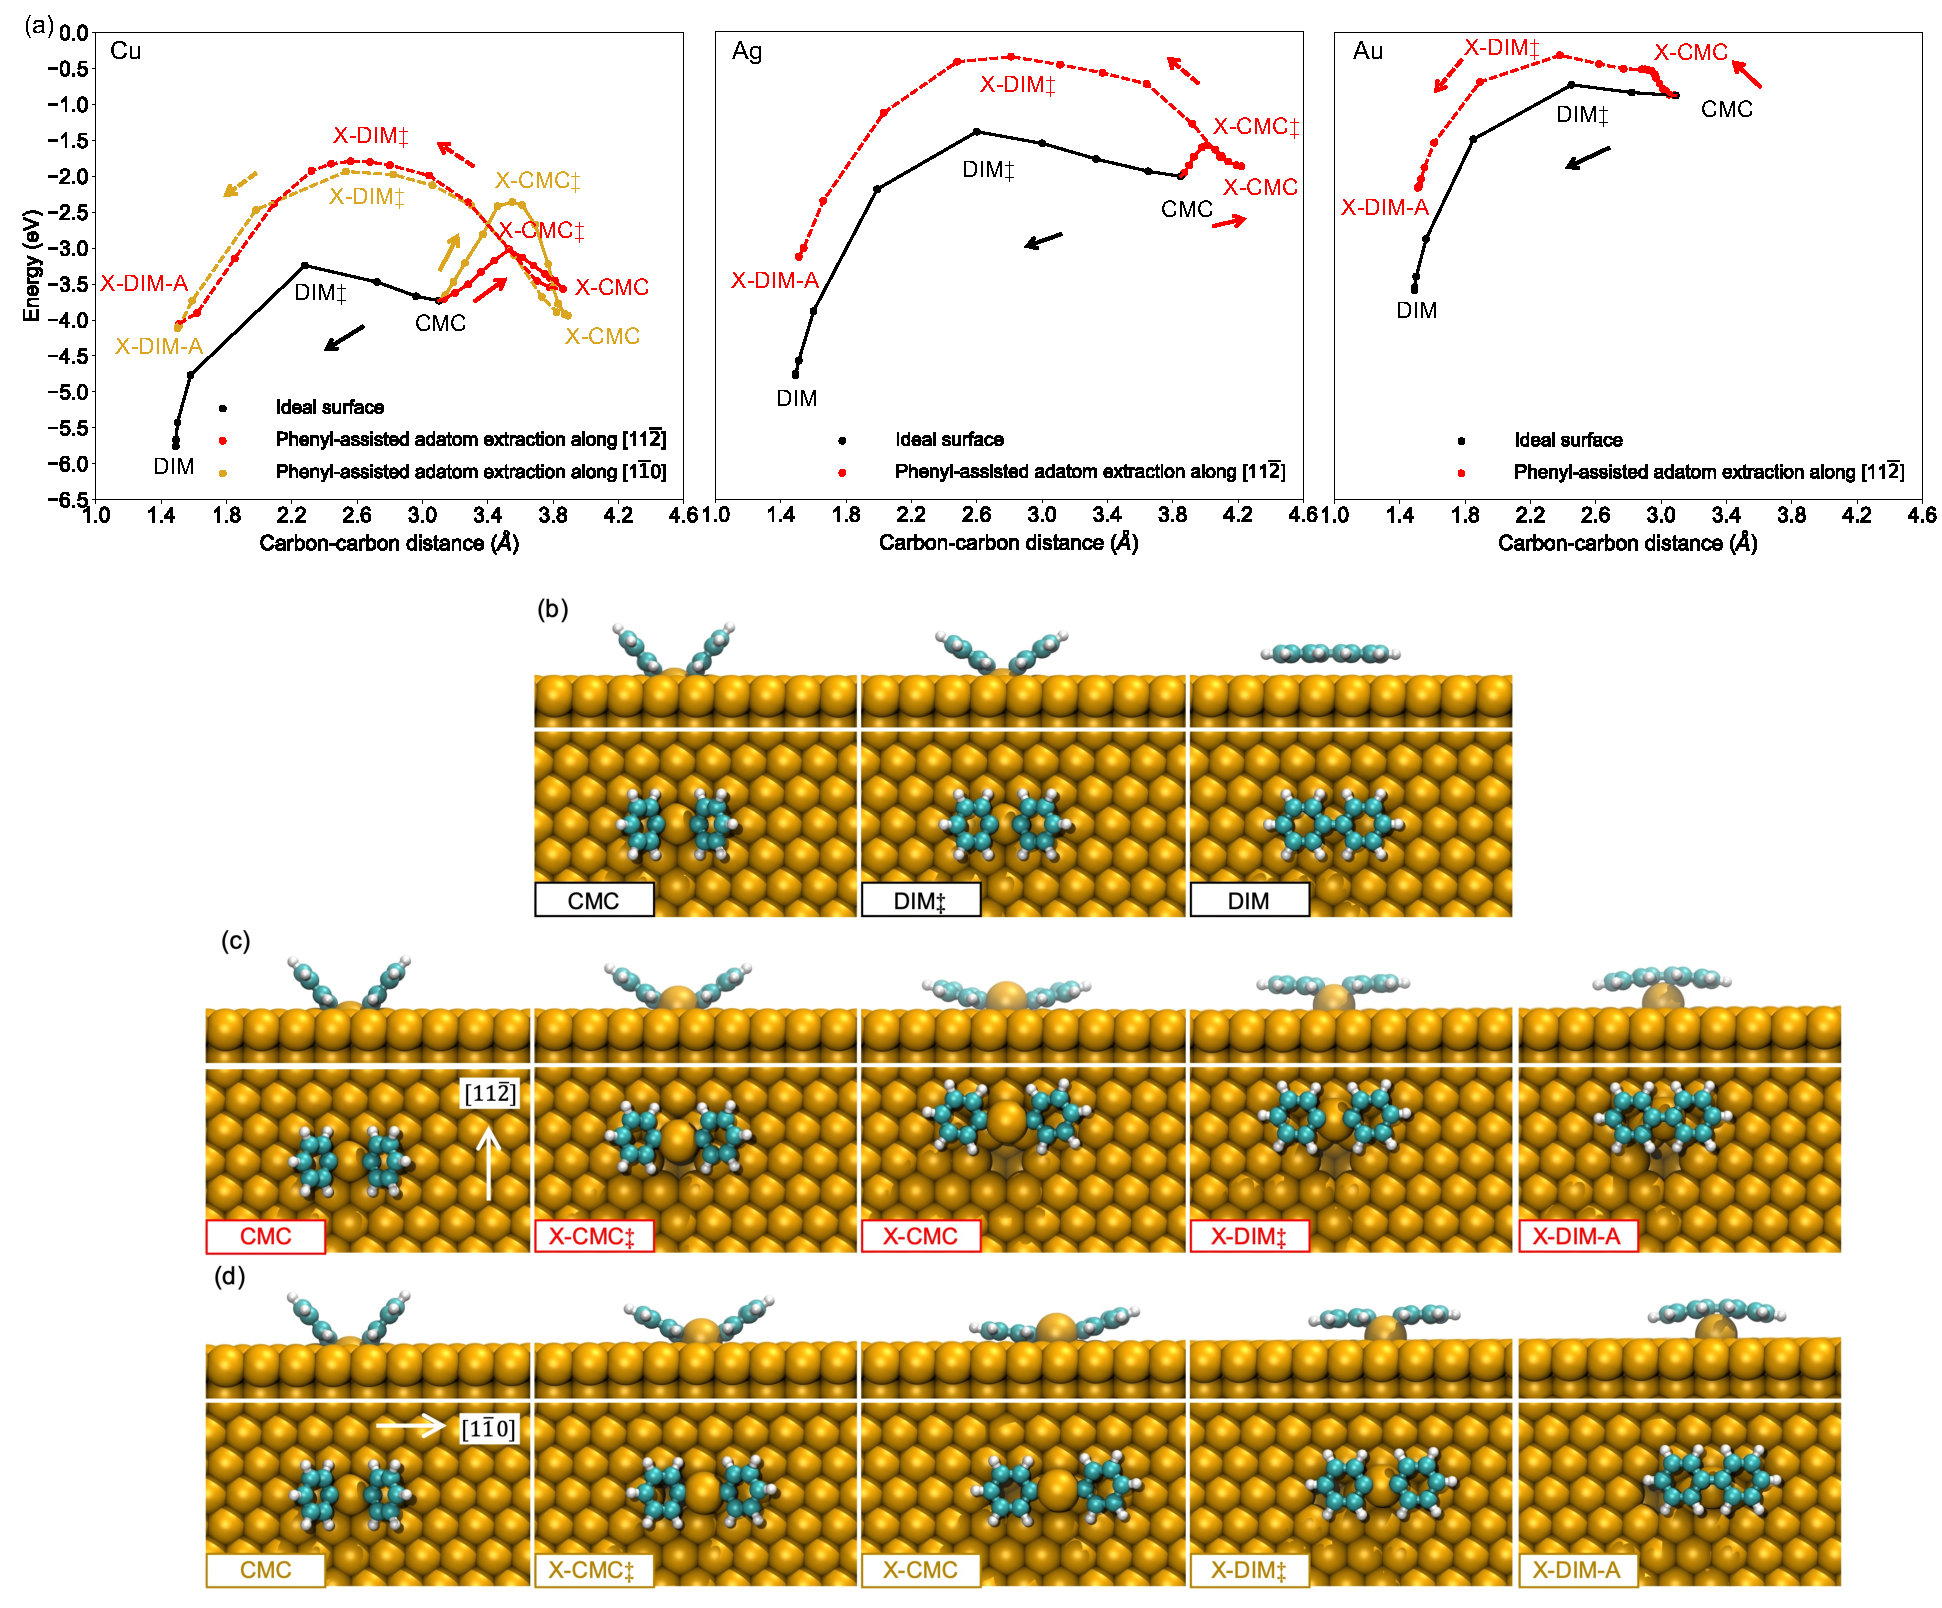
\includegraphics[width=1.0\textwidth]{Fig/distance-energy.pdf}
\caption{(a) NEB energy diagram of ideal surface path, created adatom path with longitude and latitude extraction orientations. Left is energy change vs the distance between two unsaturated carbon atoms; right is energy change vs the distance between center of mass of two phenyl radicals; (b) Geometric images of ideal surface path: C-C bond formation with catalyzed copper atom returning to its original position. Side and top view of \textbf{CMC}, \textbf{DIM$\ddagger$} and \textbf{DIM} in as labeded in Fig.~\ref{fig:completeenergy}, color representations are identical as in Fig.~\ref{fig:dissociation_Br}; (c) and (d) C-C bond formation through create adatom path. Red labels represent side and top view of extraction of adatom along [11$\overline{2}$], and yellows labels are along [1$\overline{1}$0] direction. {\comm RZK0528: Top and side views are not aligned. Align and crop.}}
\label{fig:distance-energy}
\end{figure*}

{\lock

The adatom pathway consists of three elementary steps, referred to as segments: the adatom extraction, the C--C bond formation on the adatom, and the diffusion of biphenyl away from the adatom. The two intermediates in the three-step process are denoted as \textbf{X-CMC}, \textbf{X-DIM-A}, whereas the final product is labeled as \textbf{X-DIM-B}. The first two transition states are denoted as \textbf{X-CMC$\ddagger$} and \textbf{X-DIM$\ddagger$}. The structural and energetic characteristics of the key states along the pathways are in Fig.~\ref{fig:distance-energy}, Table~\ref{table:adatom-longitude} and Table~\ref{SI-table:adatom-110} in \sinfo.

%RZK0528: Do not say "kinetically favorable", simply say "faster".
The adatom extraction along the $[1\bar{1}0]$ and $[11\bar{2}]$ surface directions were considered in this work (Fig. \ref{fig:distance-energy}). 
%
The extraction along the $[1\bar{1}0]$ direction is slightly exothermic whereas and the extraction is along the $[11\bar{2}]$ direction is slightly endothermic. It can be speculated that the \textbf{X-CMC} state is more stable in the former case because of the stronger van der Waals interaction between the undercoordinated metal atoms at the edges of the vacancy and the phenyl ring that covers the vacancy (Figure~\ref{fig:distance-energy}).
%
When the adatom is extracted along the $[1\bar{1}0]$ direction (yellow labels in Fig. \ref{fig:distance-energy}, Table~\ref{SI-table:adatom-110} in \sinfo) it moves over the top of a nearby Cu atom, whereas the adatom extracted along the $[11\bar{2}]$ direction (red labels in Fig. \ref{fig:distance-energy} and Table~\ref{table:adatom-longitude}) is shifted into the trough between two nearby atoms. Since, in the latter case, the adatom is not lifted as high in the \textbf{X-CMC$\ddagger$} transition state (\SI{1.58}{\angstrom}) as in the former case (\SI{1.68}{\angstrom}) the extraction along the $[11\bar{2}]$ direction has lower barrier (\SI{0.71}{\electronvolt} \emph{vs} \SI{1.38}{\electronvolt}). This difference in the barrier height is significant enough to consider only the $[11\bar{2}]$ extraction further.

}

\begin{figure}[hbt]
\centering
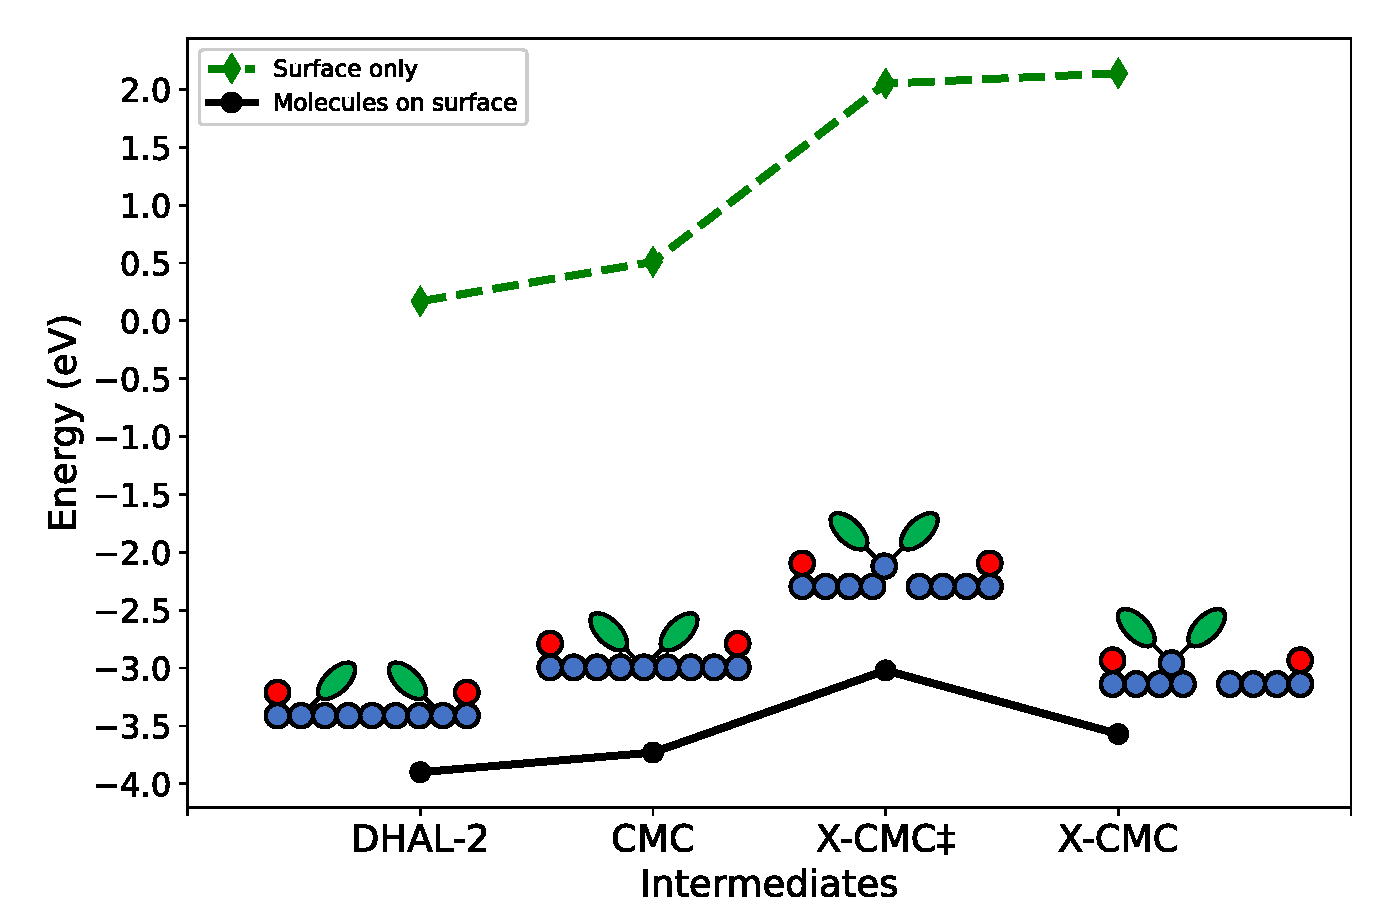
\includegraphics[width=0.48\textwidth]{Fig/onlysurface.pdf}
%\caption{Energy diagram of \textbf{DHAL-2}, \textbf{CMC}, \textbf{X-CMC$\ddagger$} and \textbf{X-CMC} from Ullmann reaction of bromobenzene, top line is the energy of isolated Cu(111) surface geometry in corresponding intermediates, and the bottom line is the energy of intermediates in Fig.~\ref{fig:completeenergy}.}
\caption{
The interaction energy between the two phenyl groups and copper atoms measured as the change from the \textbf{DHAL-2} state. Fixed copper atoms are used to estimate the interaction energy in the transition states. {\comm RZK0528: subtract black from green and plot the difference with blue color and the legend ``Fixed metal atoms''. Then use relaxed metal geometries to obtain the same line and add it with black color the legend ``Relaxed metal atoms''. Remove the old black and green lines. Include all red states: \textbf{DHAL-2}, \textbf{CMC}, \textbf{X-CMC$\ddagger$}, \textbf{X-CMC}, \textbf{X-DIM$\ddagger$}, \textbf{X-DIM-A}, \textbf{X-DIM-B}.}
}
\label{fig:onlysurface}
\end{figure}

{\lock

{\comm RZK0529: The actual number is still needed below. Re-draw the figure as requested to get the number.}
It is remarkable that the energy of the extraction of a copper atom bonded to two phenyl groups is only \SI{0.16}{\electronvolt} -- dramatically lower than the \SI{1.76}{\electronvolt} energy required to extract an adatom from the ideal clean surface (green pathway in Fig.~\ref{fig:completeenergy}). The \SI{0.71}{\electronvolt} barrier height for the phenyl-assisted extraction is also substantially lower than the \SI{2.04}{\electronvolt} barrier of clean-surface extraction.
It is suggested that the high energy cost of breaking multiple bonds between copper atoms during the phenyl-assited extraction is almost completely offset by the increased strength of binding of the phenyl groups to the extracted copper atom. This hypothesis is supported by the \SI{10000}{\electronvolt} increase in the interaction energy between the two phenyl groups and the copper atoms during the same transformation (Fig.~\ref{fig:onlysurface}). While it is difficult to separate this total interaction energy into the energy components describing $\pi$-metal and covalent carbon-adatom interaction, it is unlikely that the $\pi$-metal interaction become stronger when the phenyl rings move farther away from the surface in \textbf{X-CMC} (Fig.~\ref{fig:distance-energy}). Another argument for the stronger covalent interactions is the \SI{0.12}{\angstrom} decrease in length of the carbon-adatom bond during the \textbf{CMC} to \textbf{X-CMC} transformation (Table~\ref{table:adatom-longitude}).

It is also worth noting that the phenyl-assisted adatom extraction appears to require less energy than the previously described extraction assisted by a single phenyl group and a halogen atom, which may happen immediately after the dehalogenation step~\cite{chemeurope2017}. 
In the previous study, which used smaller slab models, optB86b exchange and local density correlation functionals, the energy of the phenyl-iodine-assisted extraction of a copper atom was calculated to be \SI{0.88}{\electronvolt}~\cite{chemeurope2017}. {\comm RZK0529: Any explanations of why iodine is less helpful?} 

With the permissive energetics of adatom extraction, it is important to look closely at the second segment of the adatom pathway, namely, the formation of the C--C bond catalyzed by the adatom. 
In contrast to the C--C bond formation on the ideal surface, the energy release along this segment of the adatom pathway is moderate \SI{-0.48}{\electronvolt} (\textit{cf.} \SI{-2.00}{\electronvolt} on the ideal surface) while the barrier height is the prohibitive \SI{1.78}{\electronvolt} (\textit{cf.} \SI{0.49}{\electronvolt}). 
This difference between the ideal-surface and adatom pathways can be attributed again to the strong bonds between the phenyl groups and adatom.
The cleavage of these strong bonds hinders the second segment of the adatom pathway as much as their formation facilitates the first extraction step. In addition to being stronger, the phenyl-adatom bonds are also likely to be stiffer (i.e. has higher vibrational frequency), further restricting the transition away from the \textbf{X-CMC} state towards \textbf{X-DIM-A}. 

It should be mentioned that the \textbf{X-DIM-B} state, in which the biphenyl is not bound to the adatom, is only \SI{0.08}{\electronvolt} higher in energy than the \textbf{X-DIM-A} state, indicating that biphenyl is not strongly bound to the adatom and and can diffuse away easily. 

From the purely thermodynamics point of view, the overall nearly thermoneutral adatom pathway (\SI{-0.24}{\electronvolt}) can be summarized as the energy released during the C--C bond formation (\SI{-2.00}{\electronvolt}) being used to extract the adatom (\SI{1.76}{\electronvolt}). The pathway of this energy redistribution is intriguingly complex with all stable states along the path -- \textbf{CMC}, \textbf{X-CMC}, \textbf{X-DIM-A}, \textbf{X-DIM-B} -- having very similar energy. First, the adatom escapes the pull of its metal neighbors with the compensating energy-releasing strengthening of the two phenyl-adatom bonds. Second, the strong C--M bonds are converted into the strong C--C bond without a significant change in energy. Finally, the biphenyl drifts away from the adatom without experiencing a strong resisting force. From the kinetics point of view, only the second segment along the path has a high energy barrier rendering the pathway inaccessible during the on-surface Ullmann coupling.

%RZZK: The energetic cost of extracting the adatom is almost completely offset by the increased binding between the two phenyl groups and the adatom in the process of extraction. The binding strength is estimated to increase by (if compared to the binding to the surface atom). Compared to adatom extraction during the DHAL step (\SI{0.88}{\electronvolt}) In this repsect adatom extrac

In addition to the C--C formation mechanism describe above, we explored an alternative pathway that proceeds from \textbf{X-CMC} directly to \textbf{X-DIM-B} without passing through \textbf{X-DIM-A}. In this pathway, the formation of C--C bond and the separation of the adatom and biphenyl happen simultaneously rather than sequentially. It was found that this path has a high activation energy of \SI{3.0}{\electronvolt} indicating that such a transformation is unrealistically slow. 
%and will not be considered further. 
%The NEB energy profile and structural changes for this segment are shown in \sinfo. RZK0528: There is no data in \sinfo.

%{\zhzh

%This path will finally reach the state where a new adatom, a vacancy spot and a biphenyl formed on copper surface. Ideally there are no interaction among these three species (\textbf{X-DIM-B}). The energy of \textbf{X-DIM-B} is increased by \SI{0.14}{\electronvolt} compared to \textbf{X-DIM-A}.
%shows trajectory from \textbf{CMC} to the C--Cu--C bridge intermediate on top of a fully extracted Cu adatom (\textbf{X-CMC}), followed by formation of dimer on this newly formed adatom (\textbf{X-DIM-A}). In \textbf{X-CMC} and \textbf{X-DIM-A}, a vacancy is generated on the original location of newly formed adatom. 
%In the first step, an Cu atom is fully extracted out in \textbf{X-CMC} bridge intermediate, energy change and barrier are \SI{-0.20}{\electronvolt} and \SI{1.38}{\electronvolt}. The distance between two carbons forming C--Cu--C bridge increases to \SI{3.89}{\angstrom} (in \textbf{X-CMC}) from \SI{3.10}{\angstrom} (iin \textbf{CMC}), and cuts down by \SI{0.34}{\angstrom} in \textbf{X-CMC$\ddagger$}. The tilt angle flattens to \SI{13}{\degree} from \SI{34}{\degree}.

%In the second step of forming C--C bond with newly formed adatom, energy change and barrier are \SI{-0.17}{\electronvolt} and \SI{2.01}{\electronvolt}. It ends with the formation of a new covalent C--C with a bond length of \SI{1.50}{\angstrom}, the former distance between these two carbons is \SI{3.10}{\angstrom} in \textbf{X-CMC}, and is condensed by \SI{0.57}{\angstrom} in \textbf{X-DIM$\ddagger$}. The tilt angle in \textbf{X-DIM-A} is a little twisted to \SI{-9.1}{\degree}. The configuration of biphenyl should be a nearly plane structure, this can be explained by the fact that the newly formed C--C is directly on the top of fully extracted Cu adatom. The distance from the Cu adatom to formed C--C bond is \SI{1.66}{\angstrom}, leading to the repulsion force and distort the two phenyl ring to such a degree.

%} %end unverified \zhzh

}

\begin{table*}
\centering\caption{Characterization of the intermediates along the $[11\bar{2}]$ adatom pathway. The states are labeled as in Fig.~\ref{fig:completeenergy}. The energies are relative to the \textbf{SURF} state.}
\label{table:adatom-longitude}
\begin{tabular}{ lccccccccccccc  }
 \hline
 \hline
  & & & Barrier & & & Change & Barrier& & &Change&\\
  & Hal. & \textbf{CMC}$^{a}$ & $\Delta^{(b-a)}$ & \textbf{X-CMC$\ddagger$}$^{b}$ & \textbf{X-CMC}$^{c}$ &$\Delta^{(c-a)}$ & $\Delta^{(d-c)}$ & \textbf{X-DIM$\ddagger$}$^{d}$ & \textbf{X-DIM-A}$^{e}$ &$\Delta^{(e-c)}$ & \textbf{X-DIM-B}  \\ 
 \hline 
 {C--C (\si{\angstrom})} & & {3.10} & {+0.43} & {3.53} & {3.86} &{+0.76} & {-1.30} & {2.56} & {1.51} &{-2.35} &{1.50}\\ 
 \hline
 {C--Cu (\si{\angstrom}) } & & {2.06} & {-0.21} & {1.85} & {1.94} &{-0.12} & {-0.05} & {1.89} & {2.16} &{+0.22} &{} \\ 
 \hline
 {Lift Cu (\si{\angstrom}) } & & {0.53} & {+1.05} & {1.58} & {1.97} &{+1.44} & {-0.16} & {1.81} & {1.71} &{-0.26} &{0.00}\\ 
% \hline
% \hline
 \hline
 \multirow{3}{*}{E (\si{\electronvolt}) } & Cl & -3.05 & +0.71 &-2.34 &-2.89 &+0.16 & +1.78 &-1.11 & -3.37&-0.48&-3.29\\ 
 & Br &-3.73 &+0.71 &-3.02 & -3.57 &+0.16 & +1.78 &-1.79 & -4.06 & -0.48&-3.97 \\ 
 & I  & -4.38 & +0.71 & -3.67& -4.22 &+0.16& +1.78 &-2.44 & -4.70 & -0.48&-4.62\\ 
 \hline
 \hline
\end{tabular}
\end{table*}

% \begin{figure*}[hbt]
% \centering
% \includegraphics[width=1.0\textwidth]{Fig/adatomall.pdf}
% \caption{C-C bond formation through create adatom path. Above images with red labels represent side and top view of extraction of adatom along longitude direction, and yellows labels below are latitude direction.}
% \label{fig:bondformadatom}
% \end{figure*}

%RZK0601: Spin density maps of the adatom-containing intermediates. Might be interesting to add.


{\lock
While the energy profile of the extraction pathway appears to suggest that the formation of phenyl-bound adatoms should be expected in the Ullmann coupling process, it is important to view these numbers in comparison to the energetic characteristics of the competitive ideal-surface pathway. Since the adatom extraction barrier is only \SI{0.22}{\electronvolt} higher than the barrier of the ideal-surface C--C bond formation the extraction process appears to happen at the relevant temperatures (\SI{350}{\kelvin} is used to promote the coupling of phenyl groups) albeit orders of magnitude slower than the ideal-surface dimerization. However, the insurmountable barrier of the second segment along the adatom pathway and the low barrier of the reversed adatom-vacancy recombination  indicate that most extracted adatoms are predestined to recombine with the vacancy and return to the \textbf{CMC} state, which eventually undergoes the irreversible ideal-surface transformation toward the biphenyl \textbf{DIM} state. This dynamics makes organometallic bridges containing extracted adatoms extremely rare, meaning that they are unlikely to be observed in STM or AFM measurements.

}

\ifdefined\INTERNAL
\subsection{Unpolished section that needs discussion}

{\zhzh

The two paths, ideal surface and create adatom are compared in multiple aspects.
As simplified geometry images in Fig.~\ref{fig:completeenergy} and NEB curves in Fig.~\ref{fig:distance-energy} indicate, two mechanisms begin to vary at \textbf{CMC}, ideal surface path (black) is thermodynamically more favourable and occurs faster than create adatom (red) due to a lower energy transition state and more stable product. This suggests that at the same temperature condition, the reaction involved in ideal surface mechanism take place at a higher speed and account for a larger percentage. In experiment, phenyl radical species require temperature at \SI{350}{\kelvin}~\cite{sur_sci01}  to accomplish C--C bonds formation on Cu(111) surface, this is more or less corresponding to a higher activation energy than \SI{0.49}{\electronvolt} obtained in ideal surface path. Even smaller energy barriers have been reported in previous work\cite{pccp2010, jacs2013}, it may come from the fact that DFT calculation provides electronic energy, instead of free energy reflecting more authentic reaction condition.

However, the evidence in geometry supports the other mechanism. In experiment, the distance between two unsaturated carbons in C--Cu--C bridge structure is \SI{4.5}{\angstrom} \textpm\ \SI{0.6}{\angstrom} based on the STM image of this bridge intermediates. This corresponds to the distance in \textbf{X-CMC} of creating adatom path, which is \SI{3.89}{\angstrom}, rather than it in \textbf{CMC} (\SI{3.10}{\angstrom}). Geometric information illustrates that create adatom path is highly likely to be occurred in experiment, which seems potentially in conflict with energetic data.

Taking the experimentally \SI{350}{\kelvin} condition for C--C bond formation and our DFT results into consideration, the ideal surface can proceed smoothly to the end, the extraction step of creating adatom is also allowed to fulfill, and then stuck at \textbf{X-CMC}, hardly to complete the coupling and form biphenyl with \SI{1.78}{\electronvolt} barrier at such condition, which explains the observation of \textbf{X-CMC} geometry. In reality, it can be inferred that \textbf{CMC} and \textbf{X-CMC} are both appeared on Cu(111) under room temperature. Upon higher annealing, \textbf{X-CMC} is mostly reverse to \textbf{CMC} and form biphenyl through ideal surface mechanism. 

In conclusion, the adatom can be created in on-surface Ullmann reaction on a defect-free Cu(111) by halobenzene due to our results, but it stagnates at organometallic states instead of achieving the final product, most biphenyl can only be formed through ideal surface mechanism.

}
\fi

%REVIEW only
\ifdefined\INTERNAL
\subsection{Desorption of products}

{\lock

The detachment of the products of the Ullmann coupling has been observed in temperature programmed desorption experiments. Biphenyl desorps from Cu(111) surface at \SIrange{400}{450}{\kelvin}, nearly \SI{100}{\kelvin} higher than the coupling temperature~\cite{ullmann_104}. Bromine and iodine atoms start to desorb at temperatures higher than \SI{900}{\kelvin} and \SI{800}{\kelvin}, respectively~\cite{jacs2013, ullmann_104}. 
In qualitative agreement with these experiments, the calculations indicate that the desorption energy of biphenyl is \SI{+1.72}{\electronvolt}, higher that the RZK energy barrier of the C--C bond formation. The calculated desorption energy of halogen atoms {\comm as diatomic molecules?} is substantially higher: \SI{+4.08}{\electronvolt} for bromine and \SI{+3.95}{\electronvolt} for iodine. 
{\comm RZK0525: As I suggested before, the energy of PROD state must be calculated with Halogen$_2$ molecule, not two separate atoms. This means that out calculations desorb holgen atoms as molecules, not as atoms.}

High desorption energy of halogen atoms is undesirable in practical on-surface Ullmann reactions. These atoms remain on metal surfaces and impede the diffusion process, which is required to couple two aryl groups. Removing the halogens can effectively optimize the speed of the process and improve the quality of synthesized polymers.

}
\fi

%%% Early steps
%R1111: LATER. Do we need adatom calculations for TS1? Perhaps only one or two halogen-metal pairs (for complete diagram). How will it affect the subsequent steps? Will the PH-Adatom roam the surface together before encountering the second Ph? PRIORITY6.

%R1111: Why there is no Cu-atom lifting during the C-X bond dissociation? Compare to previous works. Actually partial lifting is a process with a barrier for Au and Ag surfaces but not for Cu. We might need to reproduce this after all. --> More comparison to the existing calculation is required.

%RZK1222: This important effect needs to be properly described. The height of TS2-1 means that IM5, once formed will not undergo the C--C bond formation and can be viewed as an undesirable by-product of the reaction (unless it exists in quick equilibrium with IM4, which can be entropically hindered -- hard to find that vacancy again).

%RZK1222: How difficult is it to push the adatom (with attached organic radicals) DOWN into ideal surface?

%REVIEW only
\ifdefined\INTERNAL
\subsection{Coupling on an existing adatom}
\fi

{\lock

\textbf{Coupling on an existing adatom.} The shape of the energy profile along the adatom pathway is also relevant for the coupling catalyzed by the adatoms that are not extracted during the reaction but already exist on Cu(111) surface. Such pre-existing adatoms are known to form due to thermal fluctuations on the ideal surface and more often around various defects such as steps and kinks. Fig.~\ref{fig:adatomullmann} shows that, once the dehalogenation step is complete, the Ullmann coupling with pre-existing adatom is a highly exothermic process. It consists of the phenyl radicals overcoming only a minor diffusion barrier~\cite{pccp2010} to move closer to the existing adatom and to form bonds with them. Fig.~\ref{fig:adatomullmann} shows that the first phenyl is coordinated with the energy release of \SI{0.49}{\electronvolt} and the second with the release of additional \SI{0.95}{\electronvolt}. After reaching the state with two phenyl groups bonded to the adatom, the system system becomes trapped in this state. On one hand, the Ullmann coupling cannot proceed further toward biphenyl because of the height of the \textbf{X-DIM$\ddagger$} barrier. On the other hand, the reverse dissociation of the adatom-phenyl bond also requires high energy. For this reason, pre-existing adatoms on copper surface can hinder the Ullmann coupling process by creating the low-energy \textbf{X-CMC} configurations well-separated from both product and reactant states. For the Ullmann-based polymerization, the presence of adatoms can lead to defects in the nanostructures being assembled on the surface.
{\comm RZK0602: Insert the numbers above.} {\zhzh ZZ: added}

{\comm RZK0602: Slabs containing the surface vacancy are used to model pre-existing adatoms. OR should we fill the vacancy?}

}

\begin{figure}[hbt]
\centering
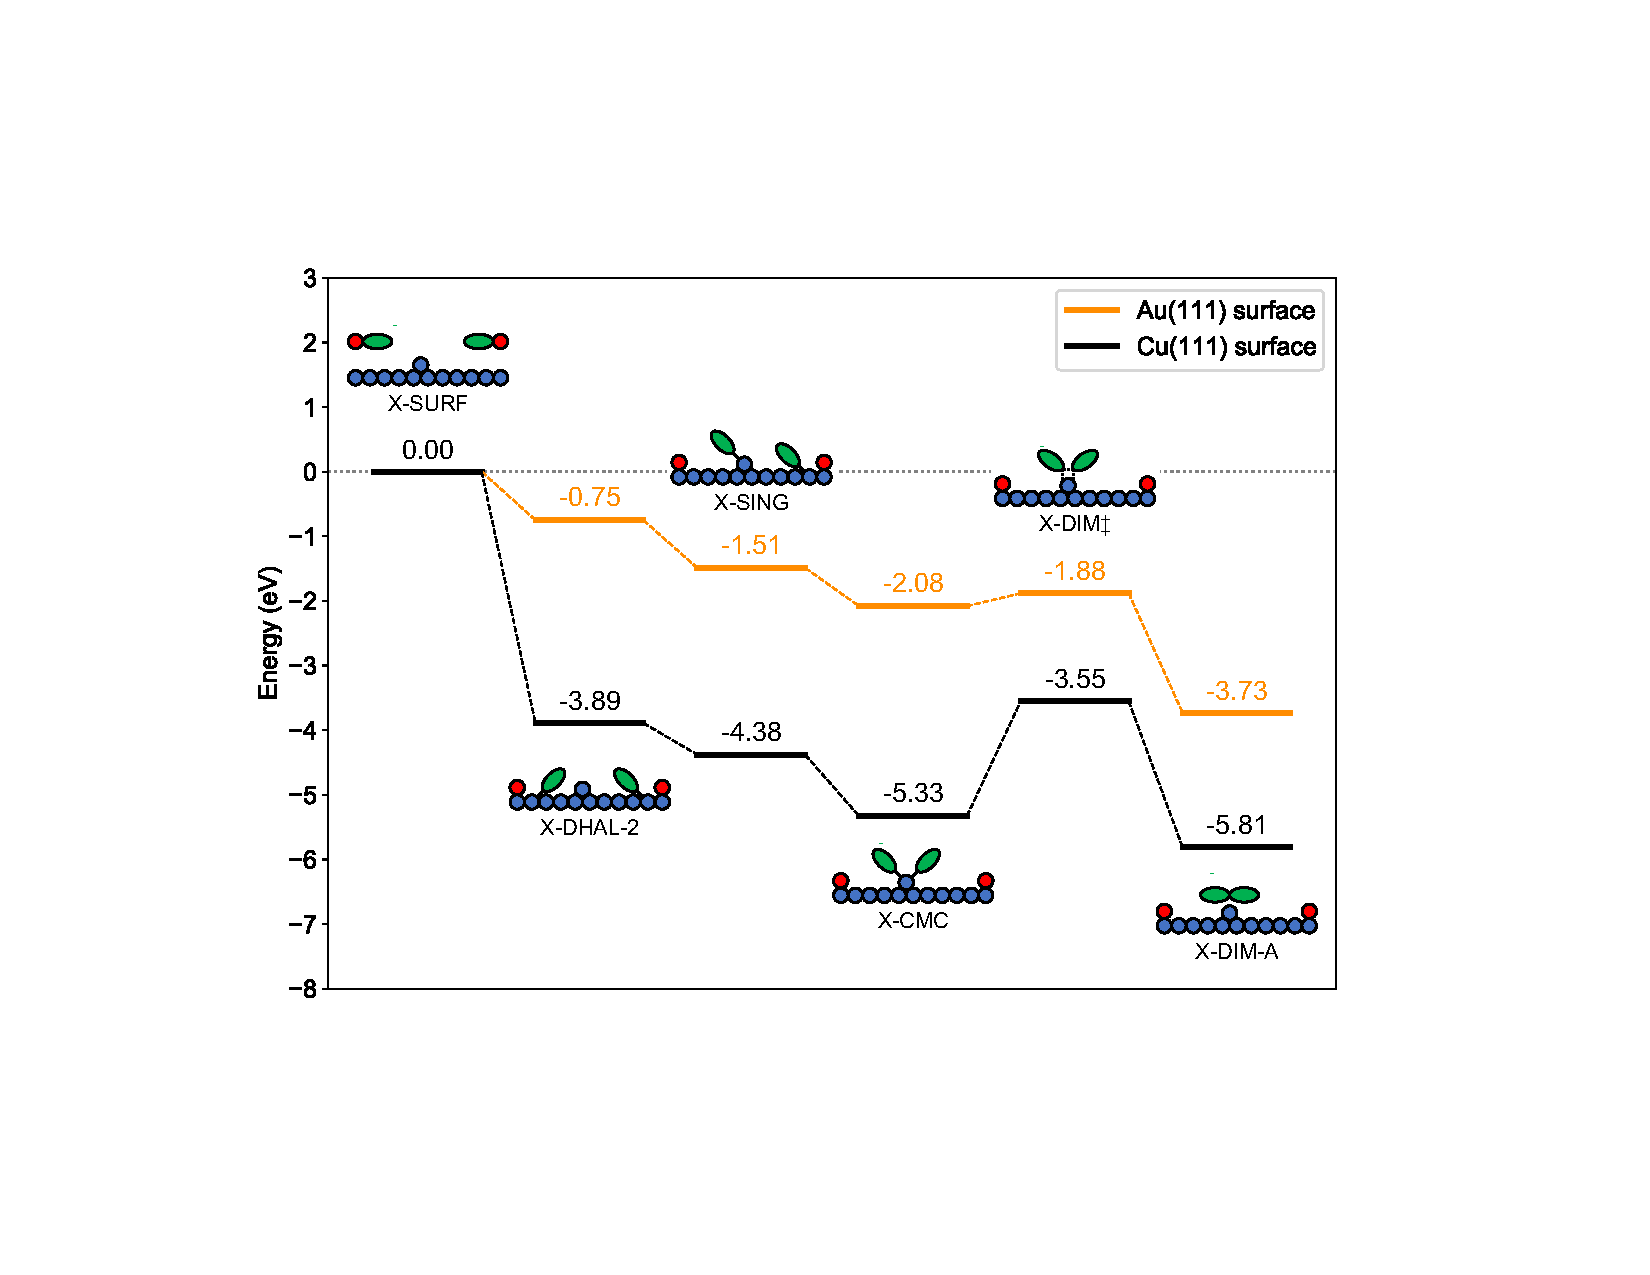
\includegraphics[width=0.48\textwidth]{Fig/ullmann_adatom.pdf}
\caption{Energy profile of the Ullmann reaction of monohalogentated benzenes on a pre-existing adatom on Cu(111) surface. The energies are relative to the \textbf{SURF} state. 
{\comm RZK0602: Energies for iodine and chlorine appears to be wrong at X-CMC and X-DIM $\ddagger$. The energy of coordinating the first and second phenyl are too different and should be verified.}
} 
\label{fig:adatomullmann}
\end{figure}

%{\comm (from Rustam) RZK0422: Can an existing adatom revert back to its original ``clean'' form to catalyze another event? It does not look plausible. First, adatom-coordinated species are anchored to the adatom too strongly to simply diffuse away. Examples. Second, adatom-coordinated species cannot react with the sufficiently low barrier to produce weakly adsorbed products. Example: C--C bond formation is hindered by the high activation barrier. C--Halogen bond formation? (ZZ: added in main text)}

\ifdefined\INTERNAL

\section{Entropy correction and free energy calculation}
{\zhzh
As mentioned, an unignorable disagreement exits between the experimental data and our DFT results. Theoretical energy barrier of dehalogenation is \SI{0.89}{\electronvolt} (\textbf{PHYS} to \textbf{DHAL$\ddagger$}), which is  higher than the energy barrier from two dehalogenated phenyls to the biphenyl (\textbf{DHAL-2} to \textbf{DIM$\ddagger$}). In experiment, C--C bond formation always requires a higher temperature to accomplish than dehalogenation step, which has been descried by the data in Table.~\ref{table:exp-temp}. This issue has also been observed in other works~\cite{jacs2013, pccp2010}. We are considering this general discrepancy arised from the ignorance of entropy in theoretical calculations. 

DFT calculations make a useful contribution to elucidating the mechanism behind the adsorption of molecules on surface, and allow precise prediction on energy and geometry. However, DFT calculations are basically limited to \SI{0}{\kelvin} temperature, describing potential energy and trend, instead of free energy change. Specifically in on-surface Ullmann reaction, the formation of dimer consists of combination of two dehalogenated species, decreasing individual mobile species as well simultaneously,  which leads to an effective decrease in entropy and make a non-negligible contribution to free energy change. Thus, to bridge the gap between experiments and simulation data in on-surface Ullmann coupling at finite temperature, entropy must be taken into consideration. 

Here the free energy diagram (Fig.\ref{fig:entropy}) is obtained after the entropy correction is done to our previous electrical energy data. Three dimensional gas molecules and two dimensional adsorbed species are both treated with transnational motion exclusively, the temperature condition for all species are at \SI{200}{\kelvin} and \SI{400}{\kelvin}, respectively. Pressure of gas molecule is $10^{-10}$ mba, which is widely used ultra high vacuum condition in on-surface Ullmann reaction, and the concentration of adsorbed molecules is \SI{10e-16}{\per\metre\squared}, which is validated by STM image~\cite{ullmann_67}. Details of derivation equations are discussed in \sinfo.

Zero energy state is fluctuated up in free energy due to including the entropy correction of gas bromobenzene. At \SI{400}{\kelvin}, the free energy barrier stay unchanged at \SI{0.89}{\electronvolt}, while the free energy barrier from \textbf{DHAL-2} to \textbf{DIM$\ddagger$} changes to \SI{1.09}{\electronvolt} from previous \SI{0.66}{\electronvolt}. The energy required for C--C coupling from two dehalogenated species has effectively increased in free energy calculations, which is further matched with the experimentally higher temperature in final step.

Our study suggests that the entropy contribution to free energy can affect the process of on-surface Ullmann coupling. The entropy calculation depends much on surface coverage, temperature and pressure, a highly consistent reaction condition parameter setup allows more accurate results in DFT calculations. It is worth to emphasize that this two dimensional lattice adsorption model is a relatively superficial, aimed at providing insight into narrowing the gap between theoretical calculation and experiment. 
}

\begin{figure*}[hbt]
\centering
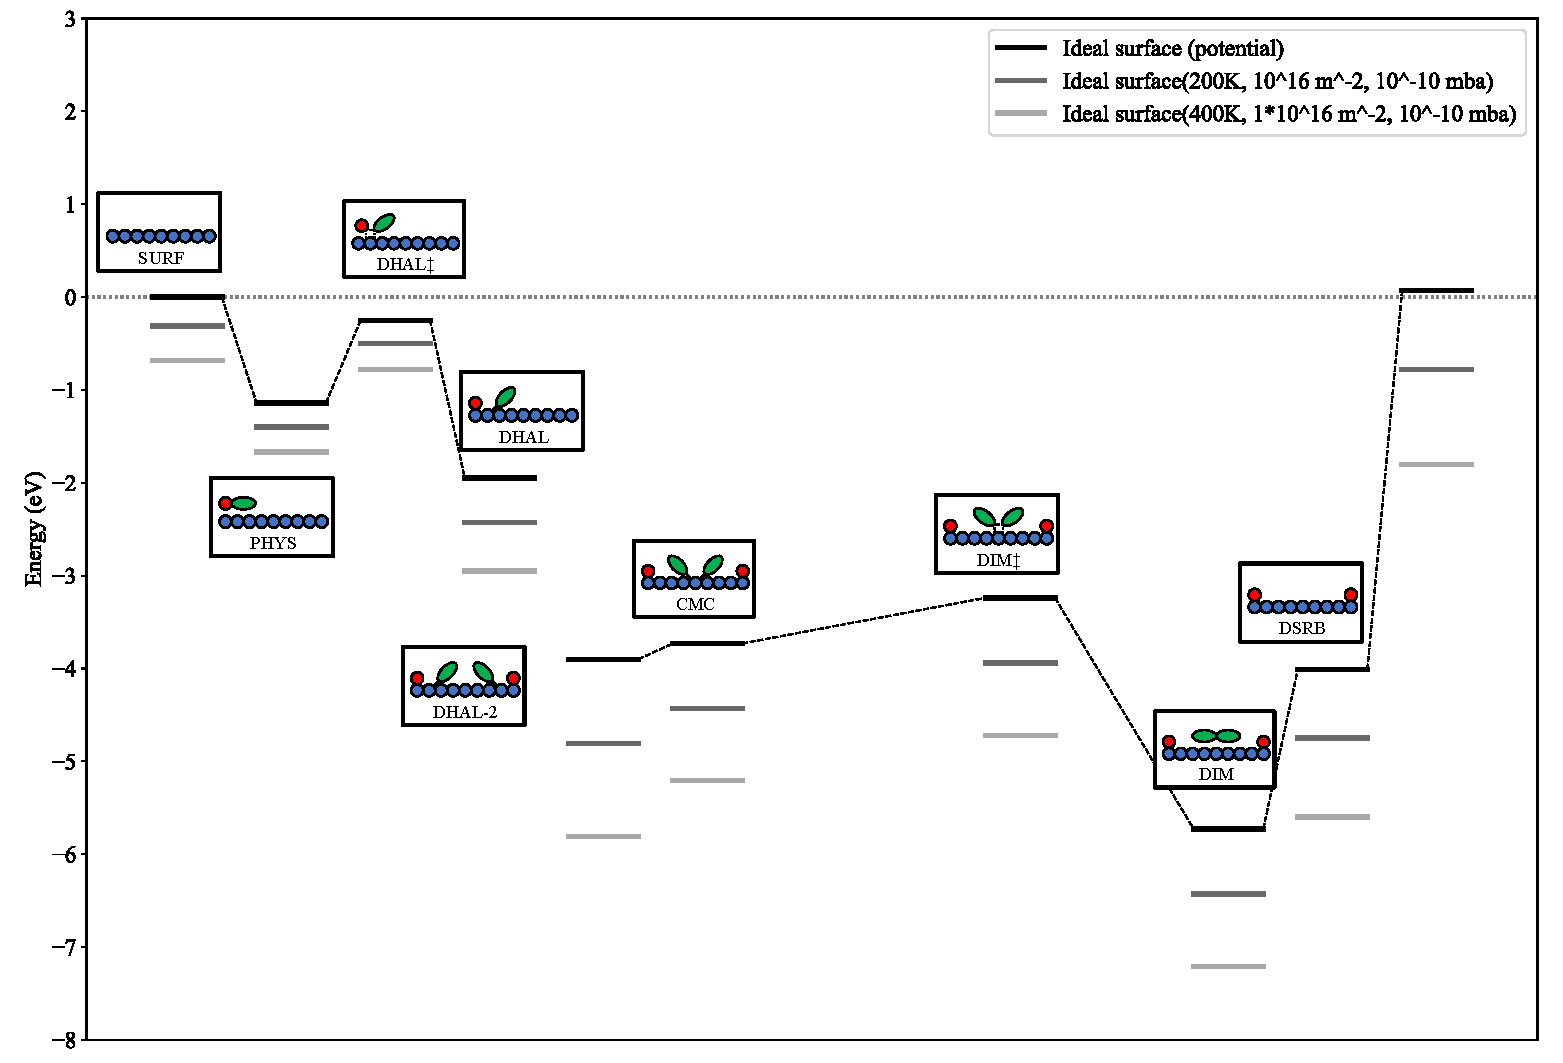
\includegraphics[width=0.98\textwidth]{Fig/entropy-correction.pdf}
\caption{The free energy diagram of bromobenzene on Cu(111) surface Ullmann coupling reaction in ideal surface path.}
\label{fig:entropy}
\end{figure*}

\fi

{\zhzh \textbf{Ullmann reactions on Ag(111) and Cu(111) surfaces.}  Coupling of bromobenzene on Ag(111) and Au(111) have been explored with the same modeling methods. 

For silver surface, debromination needs to overcome a \SI{1.20}{\electronvolt} energy barrier, \SI{0.31}{\electronvolt} higher than on copper. With formation of \textbf{CMC}, ideal-surface and adatom pathways are also compared here (only adatom extraction along the $[11\bar{2}]$ was considered). The extraction of adatom requires a \SI{0.43}{\electronvolt} of activation energy, lower than the barrier of ideal-surface pathway (\SI{0.62}{\electronvolt}). It means that the extraction of adatom is proceeding even faster than ideal surface atom catalyst on Ag(111), which is different from Cu(111). However, it also encounters the same issue as copper in the C--C bond formation step. A relatively high energy transition state \textbf{X-DIM$\ddagger$} prevents the completion of Ullmann reaction on silver, prompting the reaction reverse back and following the ideal-surface pathway as discussed above on copper surface. 

Considering three coinage surfaces, it can be inferred that adatom extraction is highly possible to occur on Ag(111) and Cu(111), nevertheless rare on Au(111) surface. This is due to that C--Ag and C--Cu bond are strong but C--Au is comparatively weak. 
}

\section{Conclusions}

%{\zhzh Thus, it can be naturally derived that there is a competition between ideal-surface atoms and adatoms which actually take part in the structure of intermediates in Ullmann coupling. Also if it is ideal-surface atoms that comprise intermediates, these ideal-surface atoms can also be fully extracted out from the first layer and become extracted adatoms, which can be regarded as an approach to create adatoms on metal surface.}

%{\zhzh For the last step, in which a C--C bond is constructed in the coupling. The role of metal atom in this formation has also been reported, but rarely compared to other steps discussed above.}

{\lock

DFT modeling was used to investigate the role of adatoms in the Ullmann coupling of monohalogenated benzenes on Cu(111) surface. It was found that the energy of the extraction of a copper atom bonded to two phenyl groups in the intermediate organometallic structure is \SI{0.16}{\electronvolt}, which is significantly lower than the \SI{1.76}{\electronvolt} energy required to extract an adatom from the ideal clean surface. In the case of the phenyl-assited extraction, the energy cost of breaking multiple bonds between copper atoms is almost completely offset by the increased binding of the phenyl groups to the extracted copper atom. This effect is also responsible for the low \SI{0.71}{\electronvolt} extraction barrier. 

Comparison of this profile to the energetic characteristics of the competing irreversible C--C bond formation on the ideal surface revealed that the extraction barrier is \SI{0.22}{\electronvolt} higher than the barrier of the C--C bond formation. This comparison indicates that the latter step proceeds faster at all temperatures and implies that the structures containing extracted adatoms can form only fleetingly in the Ullmann process. At any temperature that is sufficiently high for the adatom extraction, the equilibrium mixture will be heavily dominated by the products of the C--C coupling, making organometallic bridges containing extracted adatoms unlikely to be observed by STM or AFM.

%RZK0526: Abbreviations STM and AFM.

{\comm RZK0526: Insert the actual number below.}{\zhzh ZHZH0602: added}
The strong binding of the two phenyl groups to adatoms, which is estimated to be \SI{1.47}{\electronvolt} stronger than their binding to an ideal-surface atom, makes the barrier of the formation of the C--C bond between the adatom-bonded phenyl groups extremely high. It was calculated to be \SI{1.78}{\electronvolt} and \SI{1.29}{\electronvolt} higher that the corresponding barrier for the ideal surface reaction. This has important implications not only for the phenyl-extracted adatoms but also for the adatoms that exist on clean copper surface, for example, around steps and kinks. The presence of such a high energy barrier implies that any adatoms participating in the Ullmann reaction tend to become coordinated to phenyl groups but are unable to catalyze subsequent C--C bond formation.
%{\comm RZK0527: I think it is not only the binding strength but the stiffness of the bonds. In that case, include ``the stiff phenyl--adatom bonds''.}

{\comm RZK0527: We can discuss implications beyond the Ullmann coupling. For example, creation of adatom covered surfaces and design of ``adatom pumps''.}
%The results of this work have implications beyond the Ullmann coupling process. When it comes to design of adatom covered metal surfaces, which can serve as active catalysts for many reactions beyond the Ullmann coupling process.

}


%{\comm RZK0526: The following paragraphs need further polishing.

%The hard-to-cross peak emerges from C--C bond constructed on top of an adatom, this step will dramatically hinders the coupling to the end with biphenyl and ``clean'' adatom forming on Cu(111). In creating adatom path, two different fashions of extracting adatom out are explored and discussed. Adatom created by organometallic intermediate along the longitude direction is more likely to occur in reality due to a smaller activation energy. Plus, the heat released from the dehalogenation step is sufficient to compensate both ideal surface and create adatom paths to the end. It means ideal surface copper atom catalyze and created adatom in Ullmann process both occur in nature but occupy different proportions and proceed in different velocity.

%The possibility that adatom already emerged from thermal fluctuation or defect before the coupling is also discussed. Pre-existing adatom can be regarded as a exceedingly plausible catalyst source for organometallic intermediates in Ullmann reaction on metal surface.

%In conclusion, adatoms rarely serve as catalysts in final biphenyl formation step on Cu(111). Created adatom has a greater change to relocate in vacancy site and catalyze C--C bond with ideal surface path, ``clean'' adatom can rarely be created by dehalogenated phenyl radicals on Cu(111). 

%However, the possibility should not be ruled out, monomers with larger molecular size and stronger interaction with copper is more likely to proceed coupling to the end. This provides the insight of adatom creation by precursor design and synthesizing more 1D and 2D functional polymer through on-surface Ullmann reactions.

%{\comm RZK0525: Clean adatoms can be created if the monomers interact strongly with each other and strongly but not too strongly with the adatom. Is it possible to design such monomers? If so, will catalitically active adatoms affect the Ullmann coupling positively or negatively? Adatom creation ``machine'' can be an extremely important topics on its own, outside the fabrication of low-dimensional polymers. For example, production of super-active adatom catalysts.}

%ZZ text from objectives: And the formation of such a bridge structure can serve as a feasible strategy to create adatoms on Cu(111) surface. 

%}

% \section{surface Ullmann coupling on other coinage surface}
We have also investigated surface Ullmann coupling of bromobenzene of Ag(111) and Au(111) surfaces other than Cu(111). Ag(111) and Au(111) are modeled in the same procedure as Cu(111), 4 layers (each layer contains 48 atoms) with 20 \SI{20}{\angstrom} slab is built and optimized.




\subsection{bromobenzene on Ag(111) surface}















\subsection{bromobenzene on Au(111) surface}

%RZK. TWO follow-up projects appears to be useful. 
% 1. Explain the surprisingly low DIM activation barrier compared to DHAL activation barrier. A simple bond-strength arguments suggest that the strength of C-Metal is underestimated and possibly C-X, C-C strengths are overestimated.
% 2. Design the reaction (machine) capable of generating clean adatoms. Consider thermodynamics states of such a machine (set, grab, extract, release, leave). Consider the kinetics of the processes of switching between the states. Consider side pathways  that skip the extraction.

\section{acknowledgements}

{\lock

The research was funded by the Natural Sciences and Engineering Research Council of Canada (NSERC) through Discovery Grant (RGPIN-2016-0505) and by Tri-agency Institutional Programs Secretariat through New Frontiers in Research Fund (NFRFE-2018-00852). The authors are grateful to Compute Canada for computer time. %The authors are grateful to Compute Canada for computer resources allocated under CFI John R. Evans Leaders Fund ().

}

%\nocite{*}

\bibliographystyle{apsrev4-1} % Tell bibtex which bibliography style to use
\bibliography{references}% Produces the bibliography via BibTeX.

\end{document}








